%\documentclass[table]{article}
%\usepackage{beamerarticle}
\documentclass[10pt,xcolor=table,ignorenonframetext,handout,aspectratio=169]{beamer}
%\documentclass[10pt,xcolor=table,ignorenonframetext]{beamer}
\mode<presentation>
{
  \usetheme{default}
  \useoutertheme{split}
% \usefonttheme{serif}
}

\usenavigationsymbolstemplate{}
\usepackage{amssymb}
\usepackage{amsmath}
\usepackage{setspace}
\usepackage{graphicx}
\usepackage{multirow}
\usepackage[english]{babel}
\usepackage[latin1]{inputenc}
\usepackage{bm}
\usepackage{graphicx}
\usepackage{multirow}
\usepackage{tikz}
\usepackage[english]{babel}
\usepackage[latin1]{inputenc}
%\usepackage{ulem}
\usepackage{pifont}
\usepackage{changepage}
%\usepackage{colortbl}
%\usepackage[table]{xcolor}
%\usepackage{xcolor}

\setbeamersize{text margin left=1cm,text margin right=5cm}

\setbeamertemplate{itemize item}[circle]
\setbeamertemplate{frametitle}[default][center]

\newlength{\wideitemsep}
\setlength{\wideitemsep}{\itemsep}
\addtolength{\wideitemsep}{4pt}
\let\olditem\item
\renewcommand{\item}{\setlength{\itemsep}{\wideitemsep}\olditem}

\newcommand{\HRule}{\rule{0.5\textwidth}{0.05mm}}

\usetikzlibrary{arrows,positioning,shapes}
\usetikzlibrary{decorations.pathreplacing}
\usetikzlibrary{snakes}

\definecolor{blueish}{RGB}{97,156,255}
\definecolor{greenish}{RGB}{0,186,56}
\definecolor{reddish}{RGB}{248,118,109}

\definecolor{oiverm}{RGB}{213,94,0}
\definecolor{oiblue}{RGB}{0,114,178}
\definecolor{oigreen}{RGB}{0,158,115}
\definecolor{oipurple}{RGB}{204,121,167}
\definecolor{oiorange}{RGB}{230,159,0}
\definecolor{oisky}{RGB}{86,180,233}
\definecolor{oiyellow}{RGB}{240,228,66}
\definecolor{williams}{RGB}{81,38,152}

\definecolor{hue1}{RGB}{255,255,204}
\definecolor{hue2}{RGB}{161,218,180}
\definecolor{hue3}{RGB}{65,182,196}
\definecolor{hue4}{RGB}{44,127,184}
\definecolor{hue5}{RGB}{37,52,148}

\definecolor{dvg1}{RGB}{213,62,79}
\definecolor{dvg2}{RGB}{244,109,67}
\definecolor{dvg3}{RGB}{253,174,97}
\definecolor{dvg4}{RGB}{254,224,139}
\definecolor{dvg5}{RGB}{230,245,152}
\definecolor{dvg6}{RGB}{171,221,164}
\definecolor{dvg7}{RGB}{102,194,165}
\definecolor{dvg8}{RGB}{50,136,189}

\setbeamercolor{structure}{fg=williams,bg=williams!12}

\title{Module 6:  Diff-in-Diff in Panel Data, Slide \insertframenumber}
\subtitle{}

\author{Economics 379 (Professor Jakiela)}
\date{}



\begin{document}
	
	
	
%%%%%%%%%%%%%%%%%%%%%%%%%%%%%%%%%%%%%%%%%%%%%%%%%%%%%%%%%%%%%%%%%%%%%%%%%%
	% COURSE Title slide
%%%%%%%%%%%%%%%%%%%%%%%%%%%%%%%%%%%%%%%%%%%%%%%%%%%%%%%%%%%%%%%%%%%%%%%%%%
	
\begin{frame}<beamer:0>[plain]
	
	\begin{center}
		\begin{tikzpicture}
		
		\node [opacity=1] (bg)  {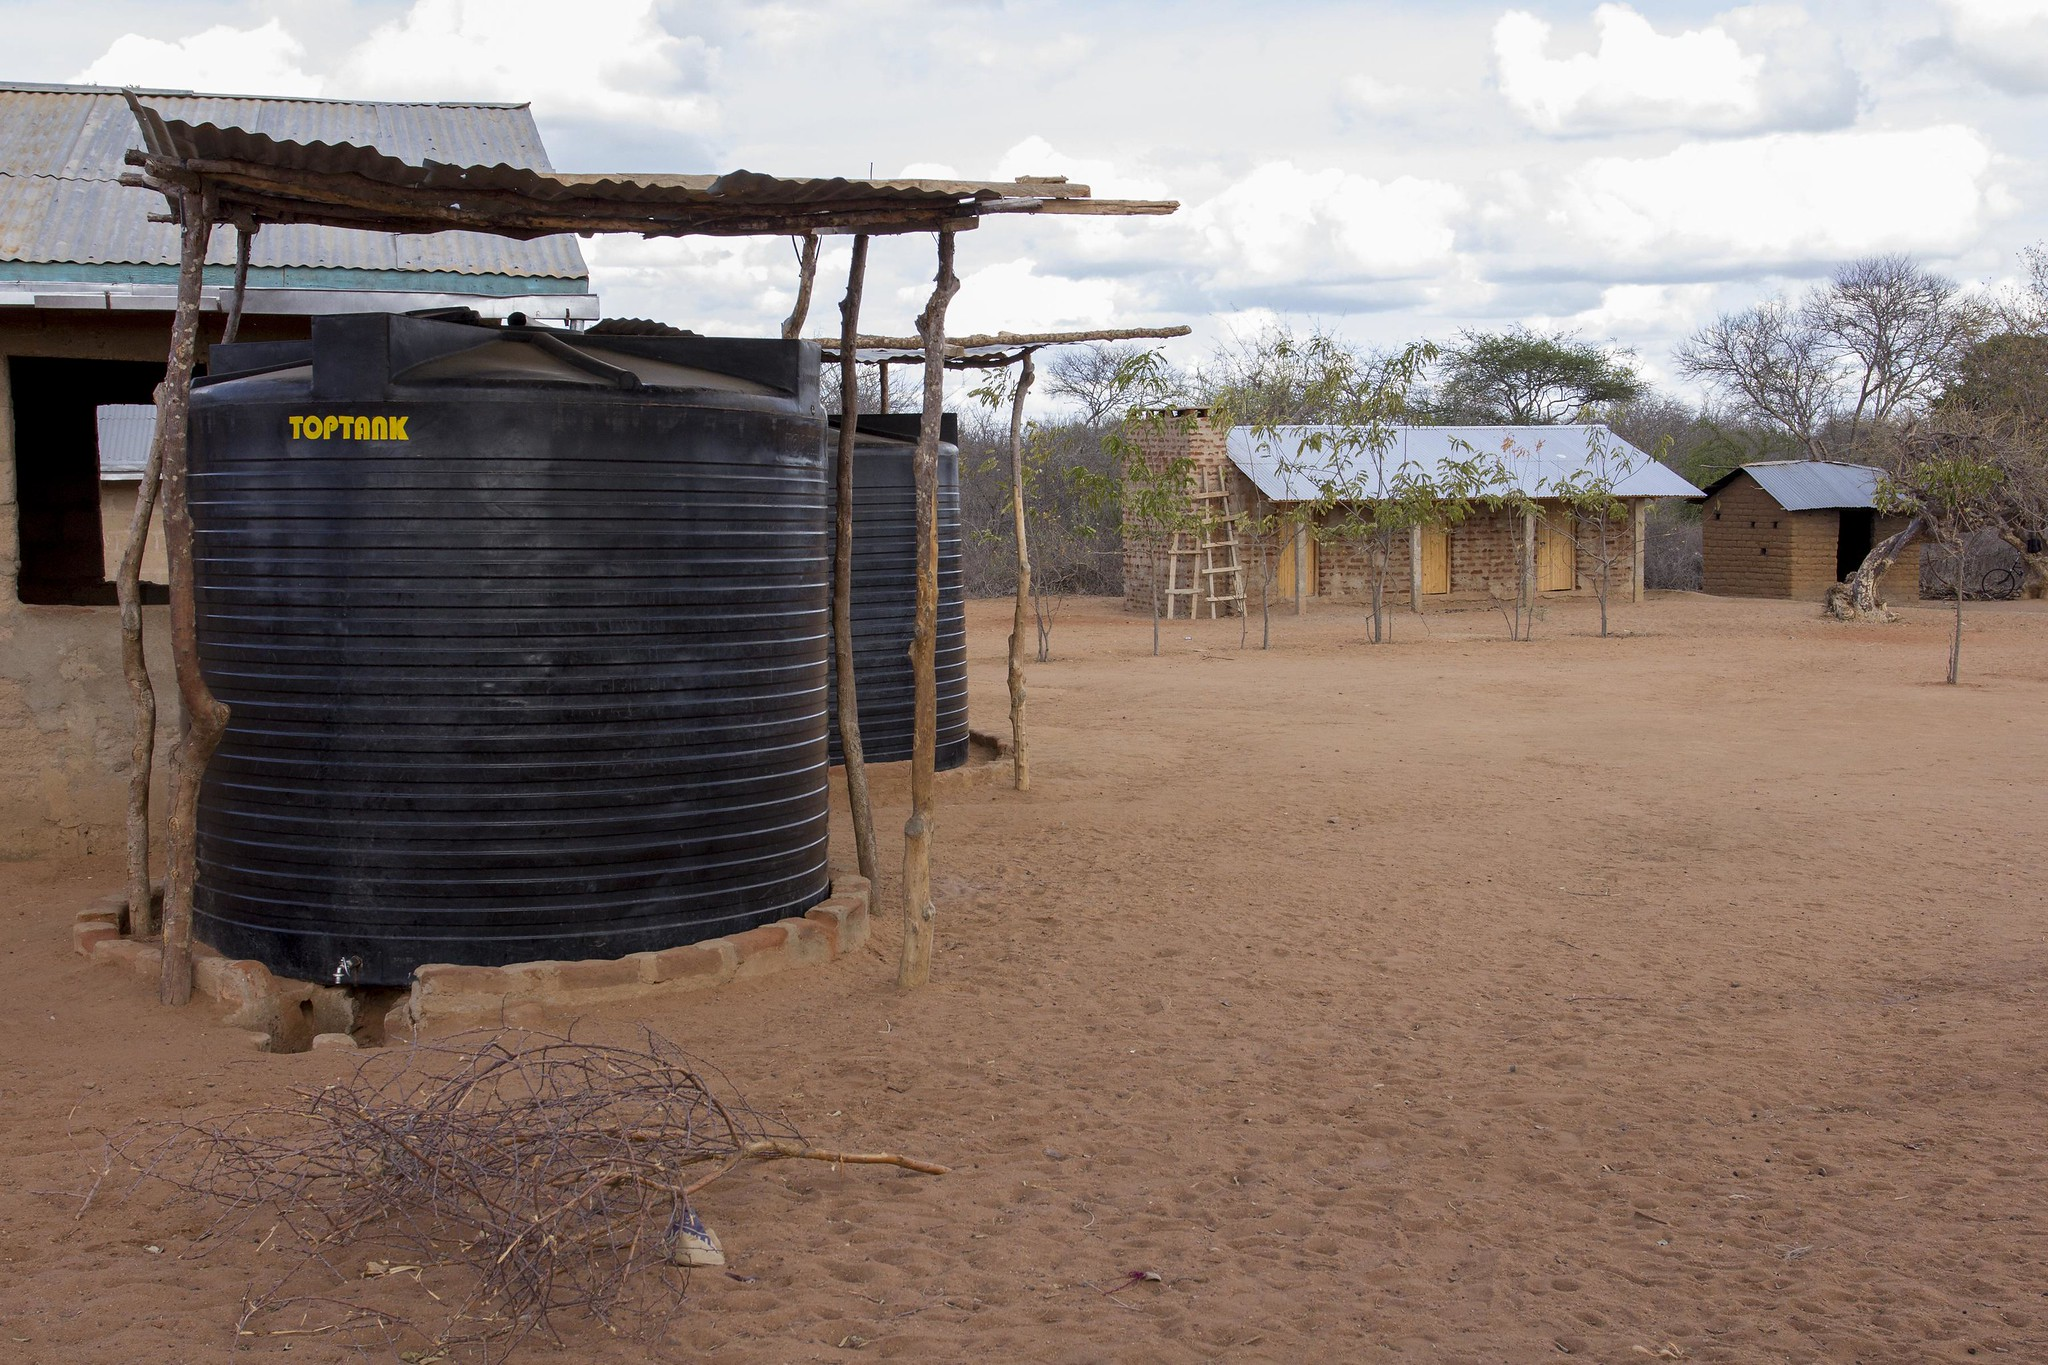
\includegraphics[keepaspectratio,height=0.9\paperheight]{photos/Kenya-cistern-Flore-de-Preneuf-2011-LARGE.jpg}};
		
		\node [anchor=east,align=right] at (6,-2.25) {\Large{\textcolor{white}{Williams College ECON 379:}}};		
		\node [anchor=east,align=right] at (6,-3) {\Large{\textcolor{white}{Program Evaluation for International Development}}};

		\node [anchor=east] at (6,-3.8) {\textcolor{yellow}{\tiny{photo:  Flore de Preneuf / World Bank}}};
		
		\end{tikzpicture}
	\end{center}
\end{frame}


%%%%%%%%%%%%%%%%%%%%%%%%%%%%%%%%%%%%%%%%%%%%%%%%%%%%%%%%%%%%%%%%%%%%%%%%%%
% LECTURE Title slide
%%%%%%%%%%%%%%%%%%%%%%%%%%%%%%%%%%%%%%%%%%%%%%%%%%%%%%%%%%%%%%%%%%%%%%%%%%

\begin{frame}[plain]

\only<beamer>{\begin{adjustwidth}{0cm}{-4cm}}

\begin{center}
	\begin{tikzpicture}
	
	\node [opacity=0.25] (bg)  {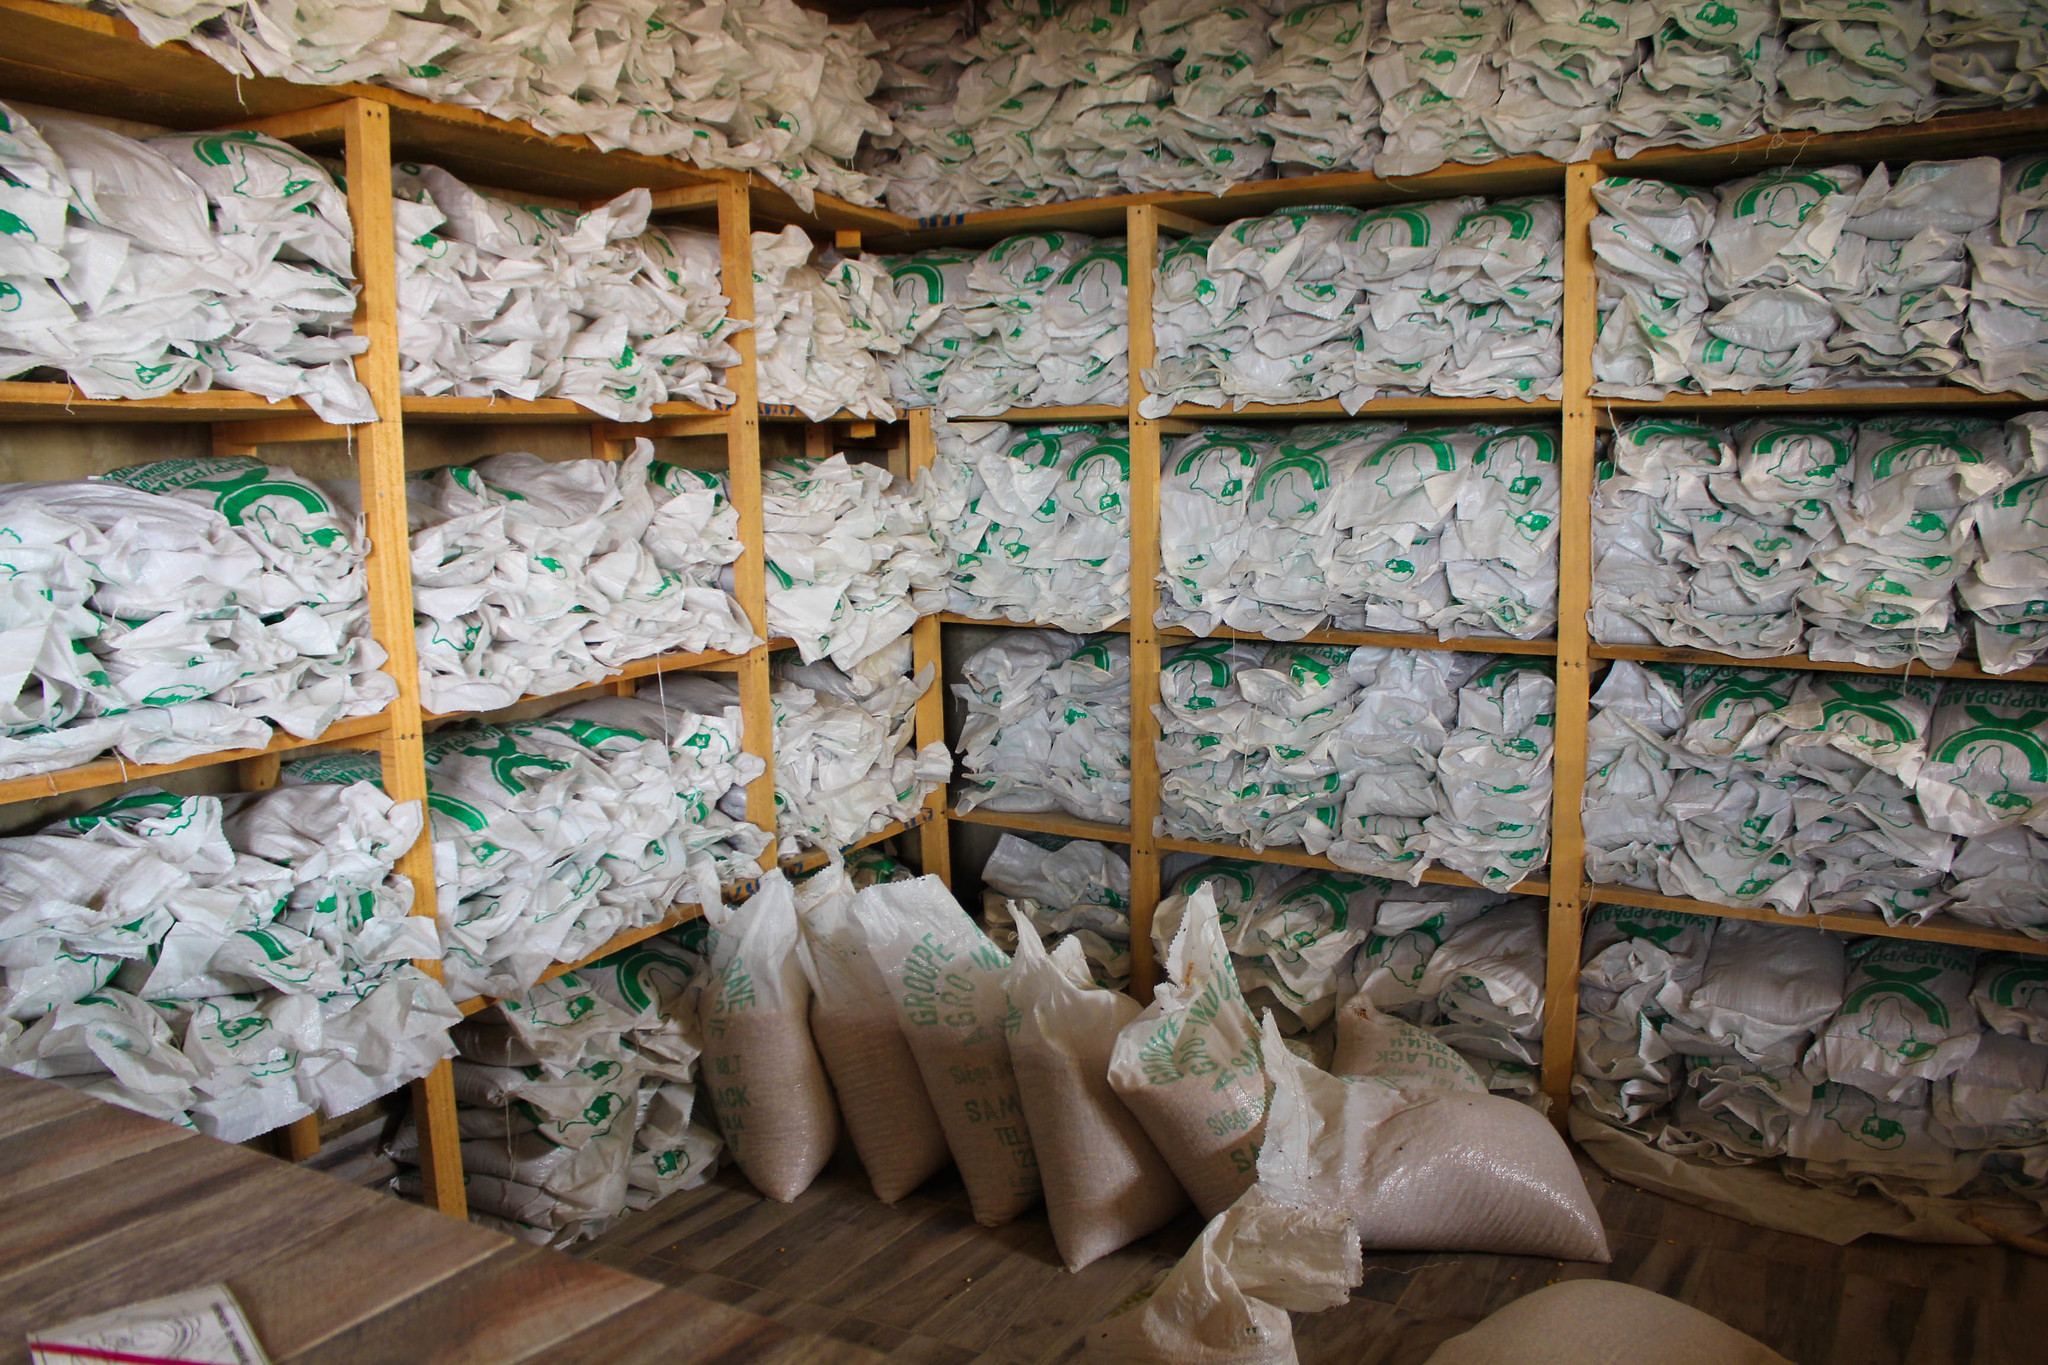
\includegraphics[keepaspectratio,height=0.9\paperheight]{photos/Senegal-WAAPP-seeds-Daniella-Van-Leggelo-Padilla-LARGE.jpg}};
	
	\node at (0,2.5) {\large{\textcolor{williams}{Williams College ECON 379:}}};		
	\node at (0,1.5) {\large{\textcolor{williams}{Program Evaluation for International Development}}};
	
	\node at (0,-0.5) {\large{\textcolor{williams}{\textbf{Module 6:  Diff-in-Diff in Panel Data}}}};
	
	\node at (0,-2) {\large{\textcolor{williams}{Professor:  Pamela Jakiela}}};
	
	\node [anchor=east] at (6,-3.8) {\textcolor{yellow}{\tiny{photo:  Daniella Van Leggelo-Padilla / World Bank}}};
	
	\end{tikzpicture}
\end{center}
\only<beamer>{\end{adjustwidth}}
\end{frame}


%%%%%%%%%%%%%%%%%%%%%%%%%%%%%%%%%%%%%%%%%%%%%%%%%%%%%%%%%%%%%%%%%%%%%%%%%%%

%\begin{frame}<handout:0>[bg,plain]
\begin{frame}[plain]

\only<beamer>{\begin{adjustwidth}{0cm}{-4cm}}
	
	\begin{center}
		
		\Large{\textcolor{williams}{Testing Common Trends}}
		
	\end{center}
	
	\only<beamer>{\end{adjustwidth}}
\end{frame}



%%%%%%%%%%%%%%%%%%%%%%%%%%%%%%%%%%%%%%%%%%%%%%%%%%%%%%%%%%%%%%%%%%%%%%%%%%%%%%%

\begin{frame}{The Common Trends Assumption}

\medskip
Diff-in-diff does not identify treatment effect if treatment and comparison groups were on different trajectories pre-program

\medskip
\begin{itemize}

\item
This is the \textbf{common trends} assumption

\smallskip

\end{itemize}

\pause
\medskip
Remember the assumptions underlying diff-in-diff estimation:

\medskip
\begin{itemize}

\item
Selection bias relates to fixed characteristics of individuals ($\gamma_i$)

\item
Time trend ($\lambda_t$) same for treatment and control groups

\end{itemize}

\pause
\medskip
These assumptions guarantee that the common trends assumption is satisfied, but they cannot be tested directly --- we have to trust

\medskip
\begin{itemize}

\item As with any identification strategy, important to think carefully about whether it checks out intuitively and econometrically

\end{itemize}

\end{frame}


%%%%%%%%%%%%%%%%%%%%%%%%%%%%%%%%%%%%%%%%%%%%%%%%%%%%%%%%%%%%%%%%%%%%%%%%%%%%%%%

\begin{frame}{How Can We Test the Common Trends Assumption?}

\medskip
A few approaches:  

\medskip
\begin{enumerate}

\item A compelling graph:  were trends similar pre-program?

\item Test equality if (linear) pre-program trends in outcome variables

\item A \textbf{placebo experiment} (or \textbf{falsification test})

\end{enumerate}

\pause
\medskip
\medskip
\textcolor{red}{Not possible with only two periods of data}

\end{frame}


%%%%%%%%%%%%%%%%%%%%%%%%%%%%%%%%%%%%%%%%%%%%%%%%%%%%%%%%%%%%%%%%%%%%%%%%%%%%%%%

\begin{frame}{Approach \#1:  A Compelling Graph}

\medskip
\begin{center}
\fbox{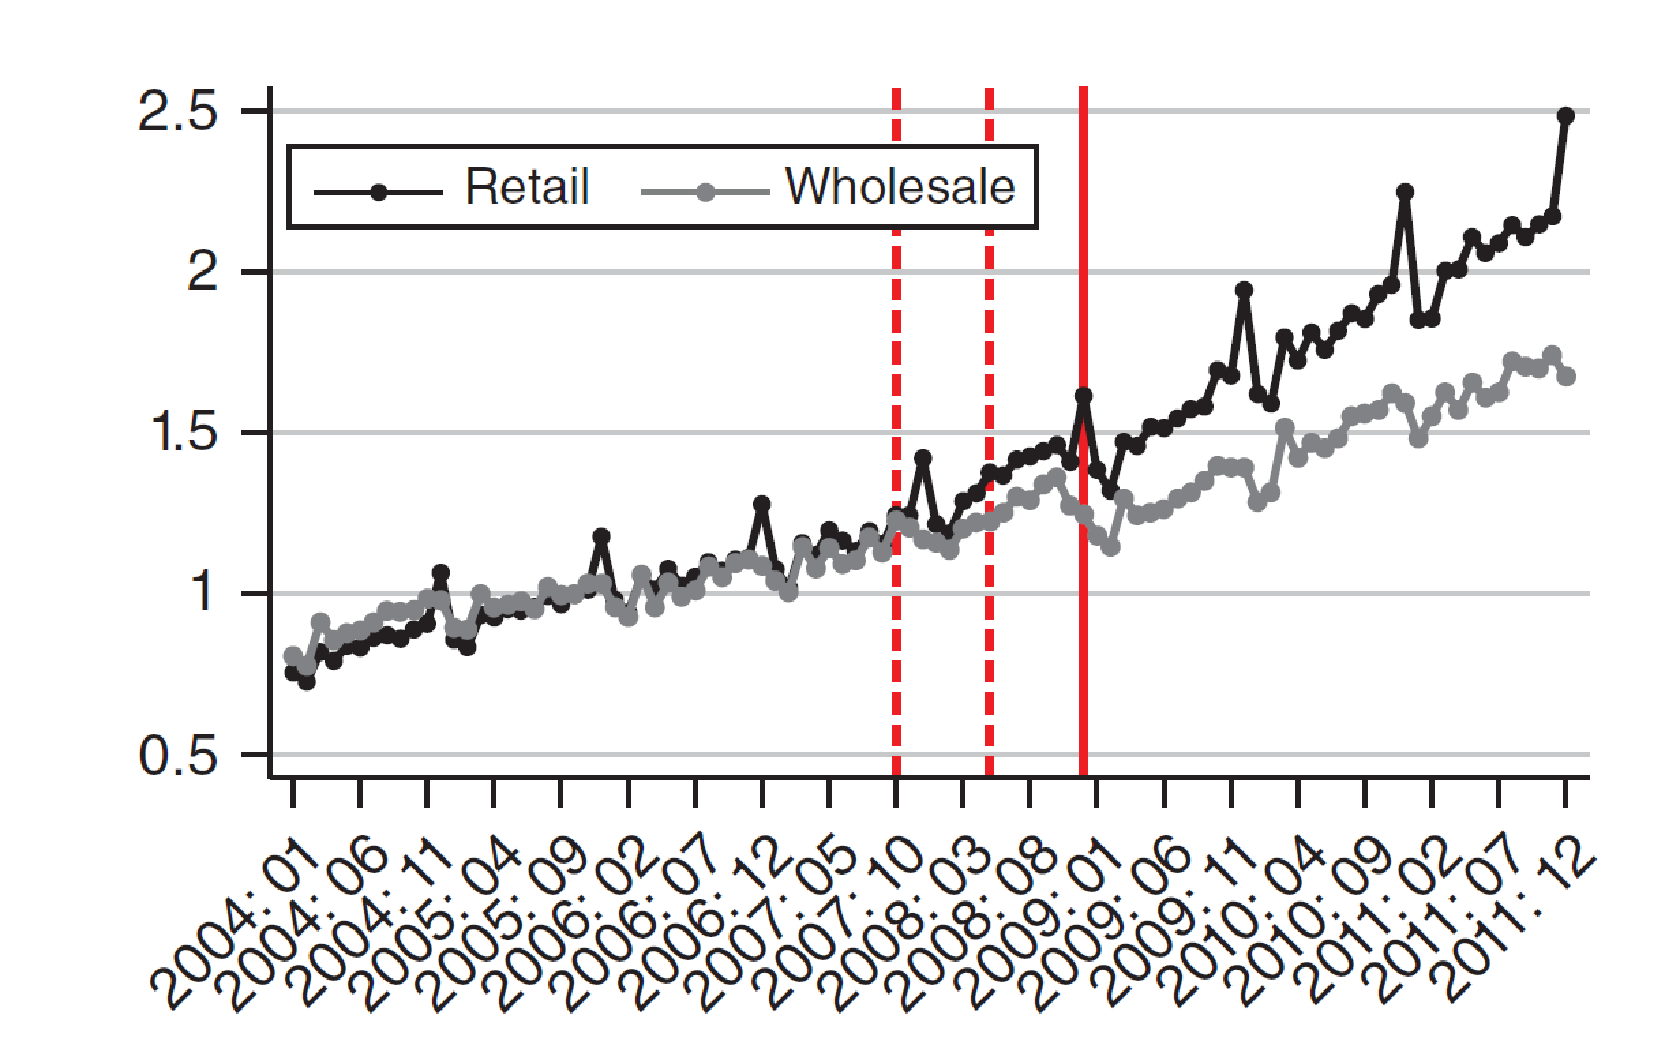
\includegraphics[width=8cm]{img/Naritomi-figure.pdf}} \\
\tiny{\textcolor{gray}{source:  Naritomi (2019)}}
\end{center}

\end{frame}


%%%%%%%%%%%%%%%%%%%%%%%%%%%%%%%%%%%%%%%%%%%%%%%%%%%%%%%%%%%%%%%%%%%%%%%%%%%%%%%

\begin{frame}{Approach \#2:  Testing Common Trends in a Regression}

\medskip
Godlonton and Okeke (2015) test for differences in pre-treatment trends:
\begin{small}
\begin{equation*}
Y_{ict} = \alpha + \beta HighExposure_c + \lambda Time_t + \gamma HighExposure_c \times Time_t   + \varepsilon_{ict}
\end{equation*}
\end{small}

\vspace{-0.5cm}

where:

\medskip
\begin{small}
\begin{itemize}

\item $Y_{it} = $ outcome variable in cluster $i$ at time $t$

\item $HighExposure_c = $ indicator for (eventually) treated clusters

\item $Time_t = $ (linear) measure of months from start of data set

\item $\gamma = $ measures equality of time trends between treatment, control

\item $ \varepsilon_{it} = $ mean-zero error term

\end{itemize}
\end{small}

\end{frame}


%%%%%%%%%%%%%%%%%%%%%%%%%%%%%%%%%%%%%%%%%%%%%%%%%%%%%%%%%%%%%%%%%%%%%%%%%%%%%%%

\begin{frame}{Approach \#2:  Testing Common Trends in a Regression}

\medskip
\begin{center}
\fbox{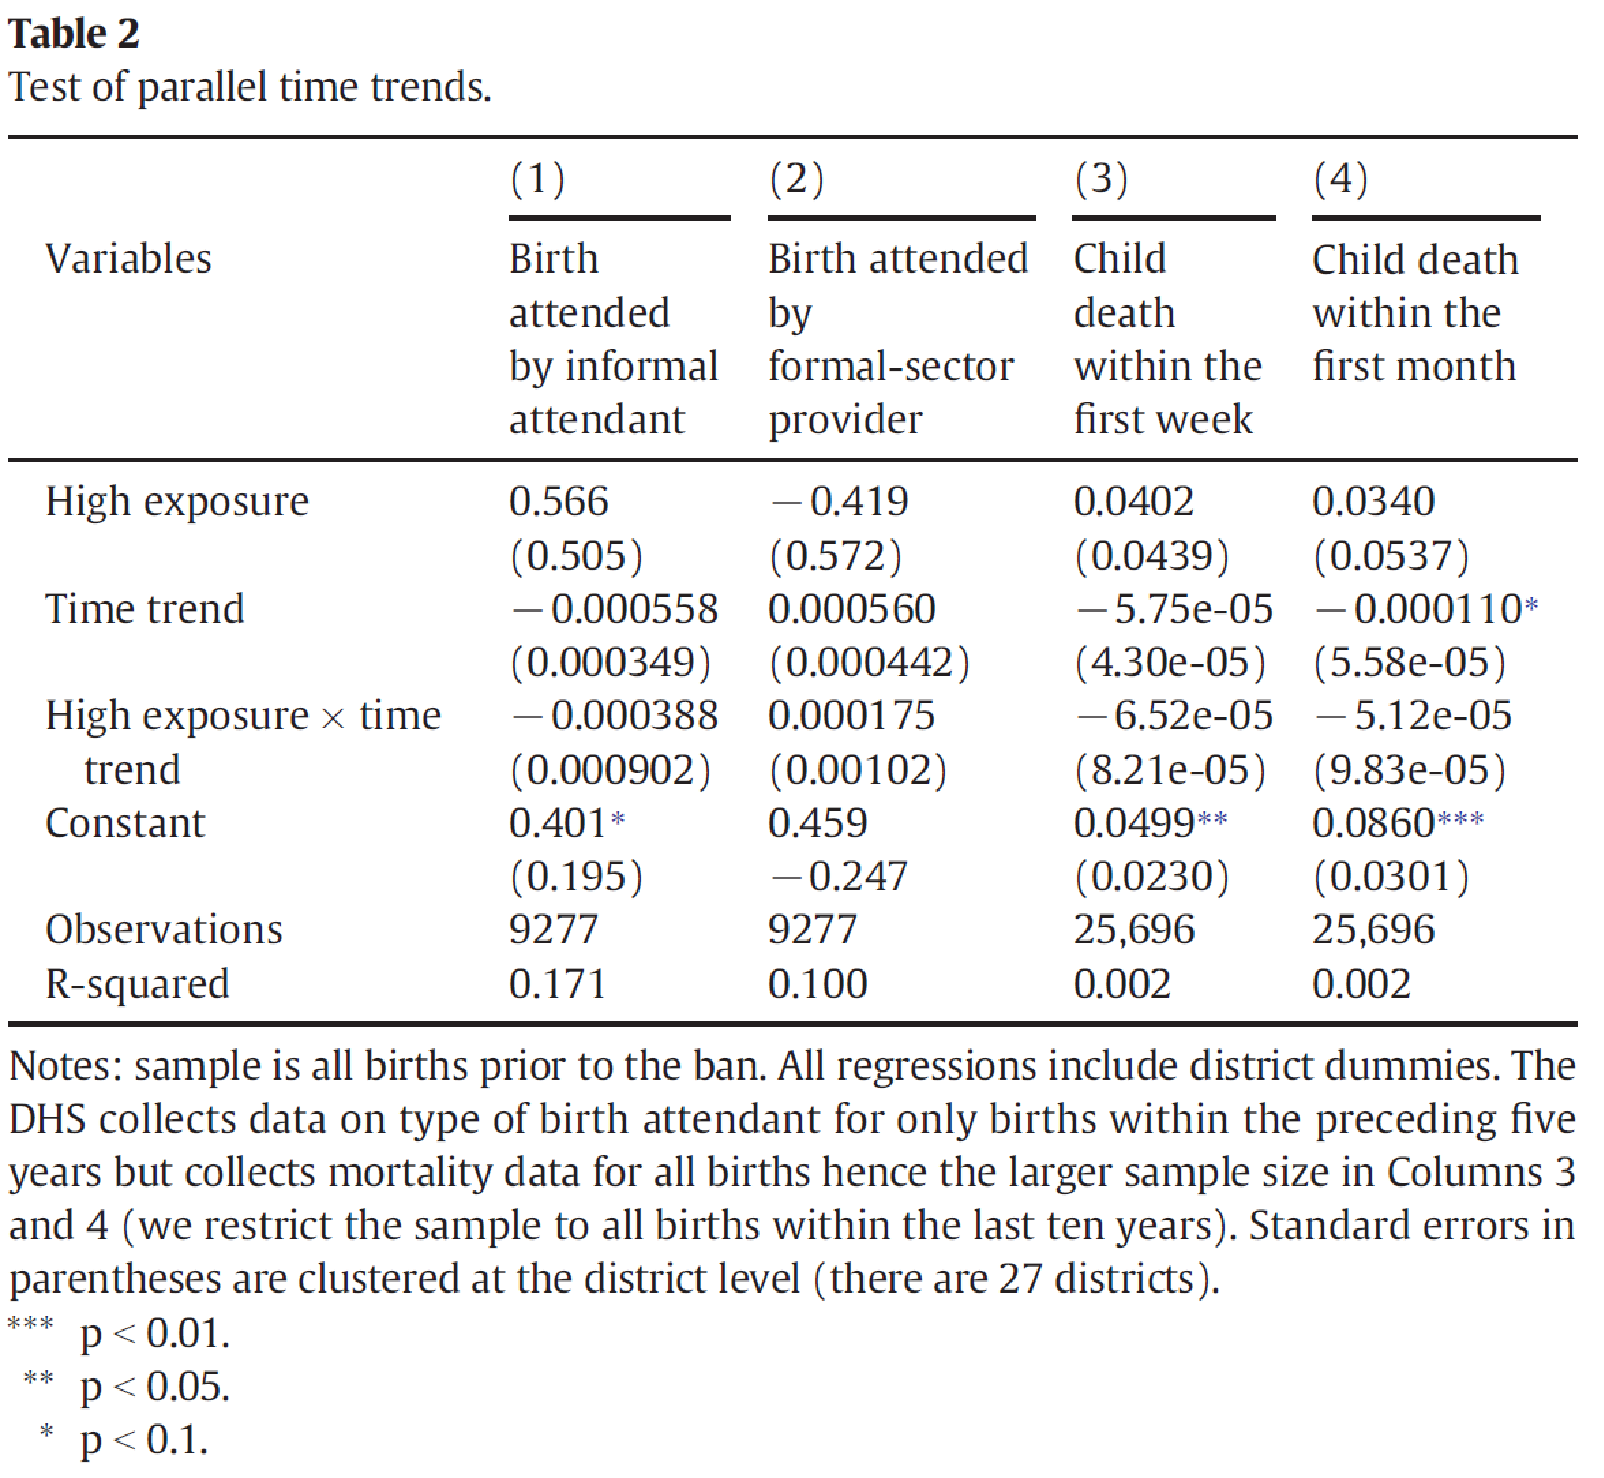
\includegraphics[height=5.2cm]{img/GO-pre-trends.pdf}} \\

\tiny{\textcolor{gray}{source:  Godlonton and Okeke (2015)}}
\end{center}

\end{frame}


%%%%%%%%%%%%%%%%%%%%%%%%%%%%%%%%%%%%%%%%%%%%%%%%%%%%%%%%%%%%%%%%%%%%%%%%%%%%%%%

\begin{frame}{Approach \#3:  A Falsification Test}

\medskip
A placebo or falsification test looks for effects that shouldn't be

\medskip
\begin{itemize}

\item In Malawi:  test whether $HighExposure_c \times Post_t$ predicts outcomes not impacted by ban on traditional birth attendants

\item In Indonesia:  test whether more schools predicts increases in educational attainment, income among (much) older cohorts

\end{itemize}


\end{frame}


%%%%%%%%%%%%%%%%%%%%%%%%%%%%%%%%%%%%%%%%%%%%%%%%%%%%%%%%%%%%%%%%%%%%%%%%%%%%%%%

\begin{frame}{Approach \#3:  A Falsification Test}

\medskip
\begin{center}
\fbox{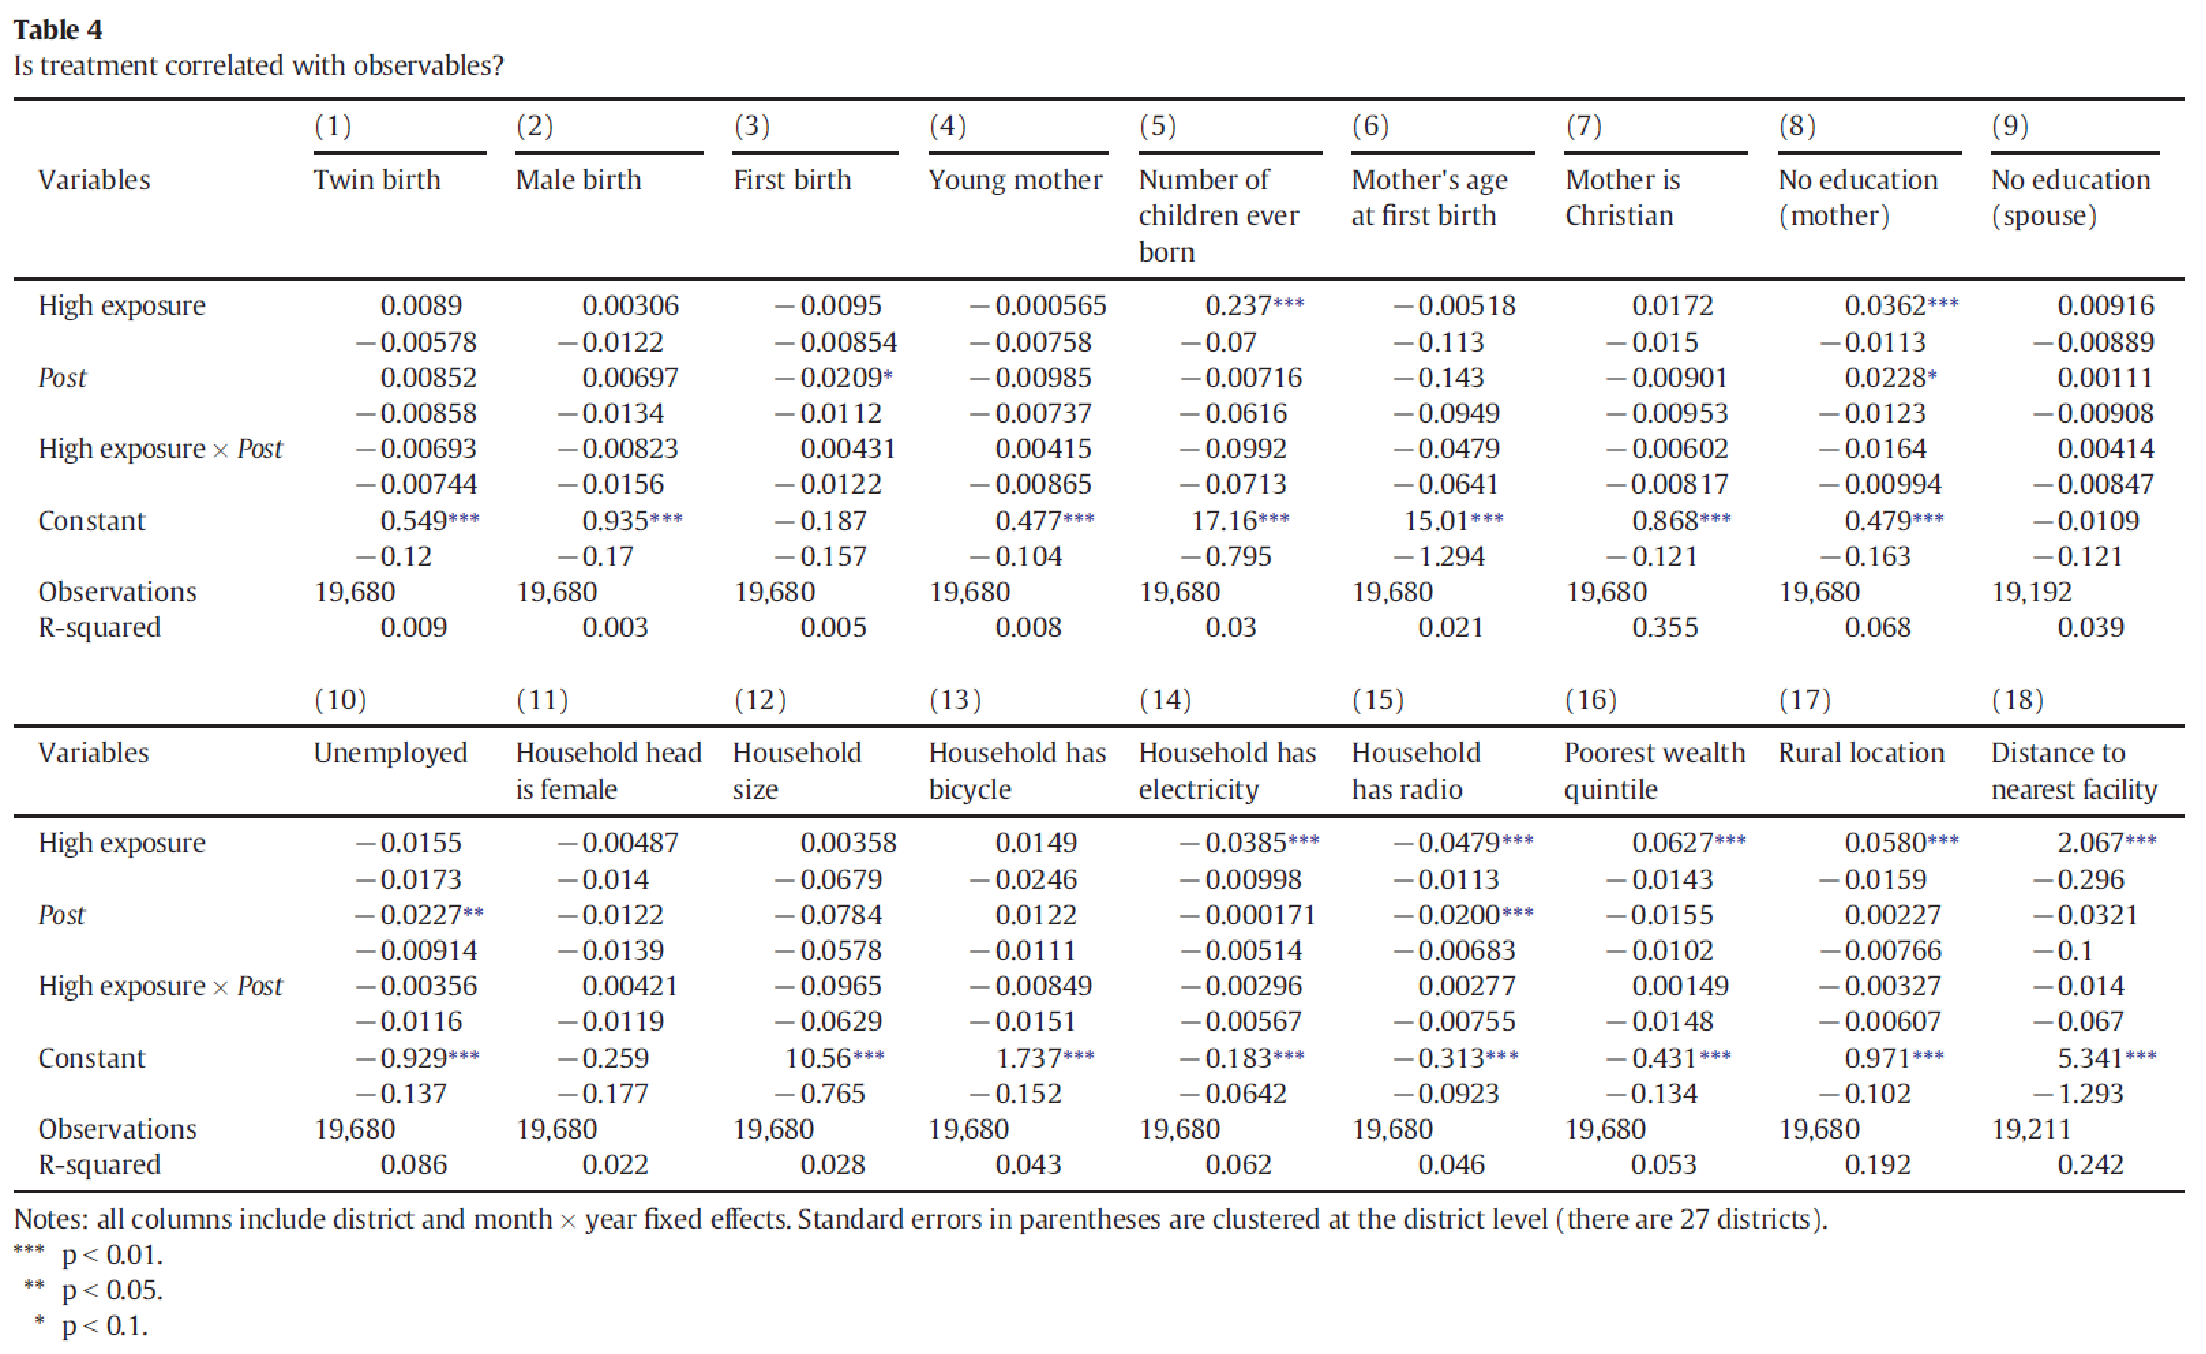
\includegraphics[height=5.2cm]{img/GO-common-trends.pdf}} \\

\tiny{\textcolor{gray}{source:  Godlonton and Okeke (2015)}}
\end{center}


\end{frame}



%%%%%%%%%%%%%%%%%%%%%%%%%%%%%%%%%%%%%%%%%%%%%%%%%%%%%%%%%%%%%%%%%%%%%%%%%%%%%%%%%%

\newpage
\begin{frame}{Approach \#3:  A Falsification Test}
\begin{center}

\fbox{\includegraphics[width=10cm]{img/duflo-NBER-figB.pdf}}\\

\tiny{\textcolor{gray}{source:  Duflo (2000)}}

\end{center}
\end{frame}


%%%%%%%%%%%%%%%%%%%%%%%%%%%%%%%%%%%%%%%%%%%%%%%%%%%%%%%%%%%%%%%%%%%%%%%%%%%%%%%

\newpage
\begin{frame}{Approach \#3:  A Falsification Test}

\medskip
\medskip
\begin{center}
\begin{footnotesize}
\begin{tabular}{lcccc}
\multicolumn{5}{c}{\textbf{Dependent Variable:  Years of Education}} \\ [0.6ex]
\hline \hline
& & & & \\ [-2.2ex]
&         & OLS   & OLS & OLS \\ [0.6ex]
& Obs.     & (1)   & (2) & (3) \\ [0.6ex]
\hline
& & & & \\ [-2.2ex]
\multicolumn{5}{l}{\textit{Panel A:  Entire Sample}} \\ [0.6ex]
$Intensity_j * Younger_i$ & 78,488    &  0.009    & 0.018 & 0.008 \\ [0.6ex]
&           & (0.026)   & (0.027)   & (0.030) \\ [0.6ex]
\hline
& & & & \\ [-2.2ex]
\multicolumn{5}{l}{\textit{Panel B:  Sample of Wage Earners}} \\ [0.6ex]
$Intensity_j * Younger_i$ & 30,255    &  0.012    & 0.024 & 0.079 \\ [0.6ex]
&           & (0.048)   & (0.048)   & (0.056) \\ [0.6ex]
\hline
& & & & \\ [-2.2ex]
\multicolumn{5}{l}{\textit{Controls Included:}} \\ [0.6ex]
YOB$*$enrollment rate in 1971   &  & No & Yes & Yes \\ [0.6ex]
YOB$*$other INPRES programs   &  & No & No & Yes \\ [0.6ex]
\hline
& & & & \\ [-2.2ex]
\multicolumn{5}{p{9.5cm}}{\scriptsize{Sample includes individuals aged 12 to 24 in 1974.  All Specifications include region of birth dummies, year of birth dummies, and interactions between the year of birth dummis and the number of children in the region of birth (in 1971).  Standard errors are in parentheses.}}
\end{tabular}
\end{footnotesize}
\end{center}

\end{frame}





%%%%%%%%%%%%%%%%%%%%%%%%%%%%%%%%%%%%%%%%%%%%%%%%%%%%%%%%%%%%%%%%%%%%%%%%%%%

%\begin{frame}<handout:0>[bg,plain]
\begin{frame}[plain]

\only<beamer>{\begin{adjustwidth}{0cm}{-4cm}}

\begin{center}
	
	\Large{\textcolor{williams}{Event Studies}}
	
\end{center}

\only<beamer>{\end{adjustwidth}}
\end{frame}


%%%%%%%%%%%%%%%%%%%%%%%%%%%%%%%%%%%%%%%%%%%%%%%%%%%%%%%%%%%%%%%%%%%%%%%

\begin{frame}{The Difference-in-Differences Estimator}

\begin{center}
	\begin{tikzpicture}
	
	% blank canvas
	\only<handout>{\fill[fill=white,draw=white,ultra thin]
	(0,0) -- (11,0) -- (11,6) -- (0,6) -- cycle;}
	\only<beamer>{\fill[fill=white,draw=white,ultra thin]
	(0,0) -- (14,0) -- (14,6) -- (0,6) -- cycle;}
	\only<beamer>{\draw[draw=oiblue!60,fill=oiblue!10,opacity=0.5] (11,1) rectangle (14,5);}
	%\draw[step=1.0,gray!20,thin] (0,0) grid (11,6);
	
%	\pgfmathsetmacro\xshift{0.5cm};
%	\pgfmathsetmacro\yshift{5.5cm};
%	\pgfmathsetmacro\mycolor{"gray"};

	\node[anchor=north] (fig) at (5,5.75) {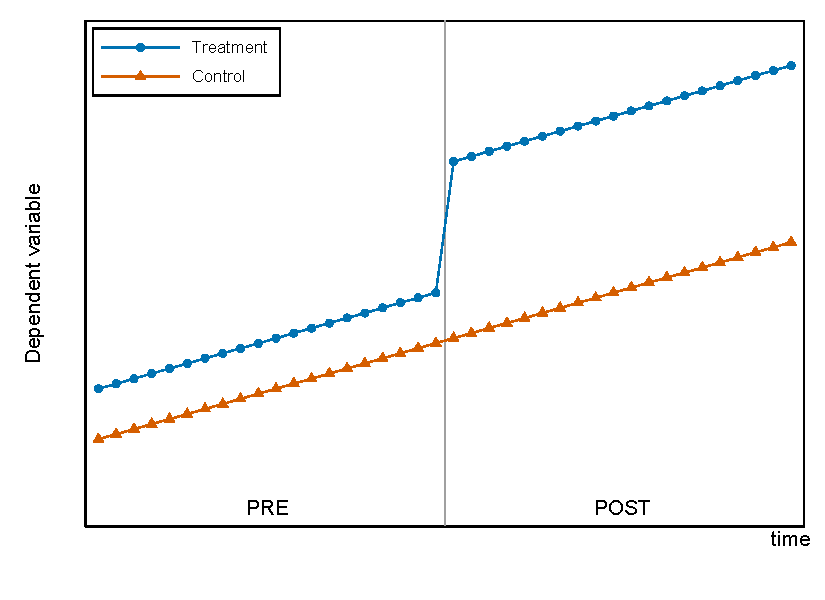
\includegraphics[height=4.0cm]{fig/plainDD1.pdf}};
	
	\node[anchor=north,align=center] (text1) at (fig.south) {Diff-in-diff estimator is a linear combination four cell means};
		
	\node[anchor=base west,align=left] (text2) at ([xshift=0.25cm,yshift=-0.625cm]text1.base west) {\structure{$\bullet$} In panel data, cell means average across periods};	
	
	\end{tikzpicture}
\end{center}
\end{frame}



%%%%%%%%%%%%%%%%%%%%%%%%%%%%%%%%%%%%%%%%%%%%%%%%%%%%%%%%%%%%%%%%%%%%%%%

\begin{frame}{The Difference-in-Differences Estimator}

\begin{center}
	\begin{tikzpicture}
	
	% blank canvas
	\only<handout>{\fill[fill=white,draw=white,ultra thin]
		(0,0) -- (11,0) -- (11,6) -- (0,6) -- cycle;}
	\only<beamer>{\fill[fill=white,draw=white,ultra thin]
		(0,0) -- (14,0) -- (14,6) -- (0,6) -- cycle;}
	\only<beamer>{\draw[draw=oiblue!60,fill=oiblue!10,opacity=0.5] (11,1) rectangle (14,5);}
	%\draw[step=1.0,gray!20,thin] (0,0) grid (11,6);
	
	%	\pgfmathsetmacro\xshift{0.5cm};
	%	\pgfmathsetmacro\yshift{5.5cm};
	%	\pgfmathsetmacro\mycolor{"gray"};
	
	\node[anchor=north] (fig) at (5,5.75) {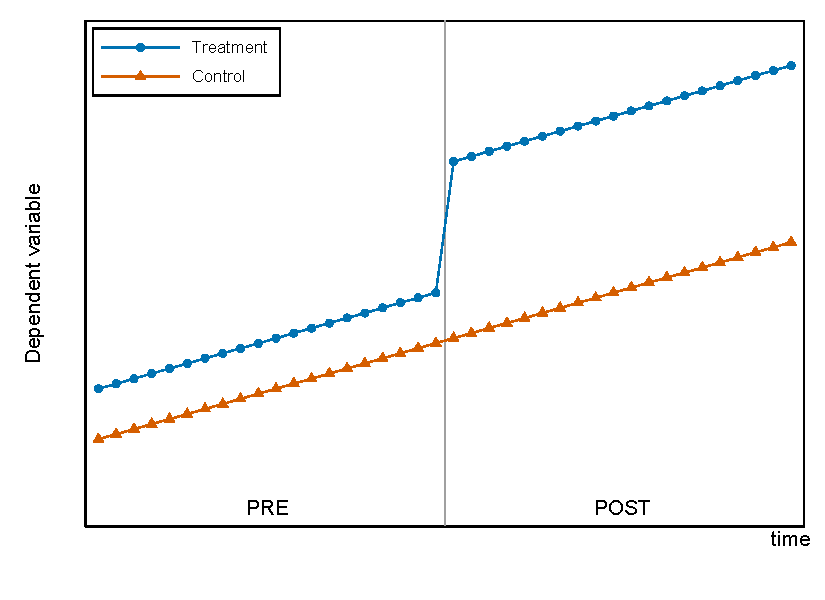
\includegraphics[height=4.0cm]{fig/plainDD1.pdf}};
	
	\node[anchor=north,align=center] (text1) at (fig.south) {Clear interpretation when treatment effect is constant};
	
	\node[anchor=base,align=center] (text2) at ([yshift=-0.625cm]text1.base) {\structure{$\Rightarrow$} $E [ Y_{it} ] = \textcolor{red}{\gamma_i} + \textcolor{red}{\lambda_t} + \delta_i D_{it} $};	
	
	\end{tikzpicture}
\end{center}
\end{frame}



%%%%%%%%%%%%%%%%%%%%%%%%%%%%%%%%%%%%%%%%%%%%%%%%%%%%%%%%%%%%%%%%%%%%%%%

\begin{frame}{When Treatment Effect Changes Over Time}

\begin{center}
	\begin{tikzpicture}
	
	% blank canvas
	\only<handout>{\fill[fill=white,draw=white,ultra thin]
		(0,0) -- (11,0) -- (11,6) -- (0,6) -- cycle;}
	\only<beamer>{\fill[fill=white,draw=white,ultra thin]
		(0,0) -- (14,0) -- (14,6) -- (0,6) -- cycle;}
	\only<beamer>{\draw[draw=oiblue!60,fill=oiblue!10,opacity=0.5] (11,1) rectangle (14,5);}
	%\draw[step=1.0,gray!20,thin] (0,0) grid (11,6);
	
	%	\pgfmathsetmacro\xshift{0.5cm};
	%	\pgfmathsetmacro\yshift{5.5cm};
	%	\pgfmathsetmacro\mycolor{"gray"};
	
	\node[anchor=north] (fig) at (5,5.75) {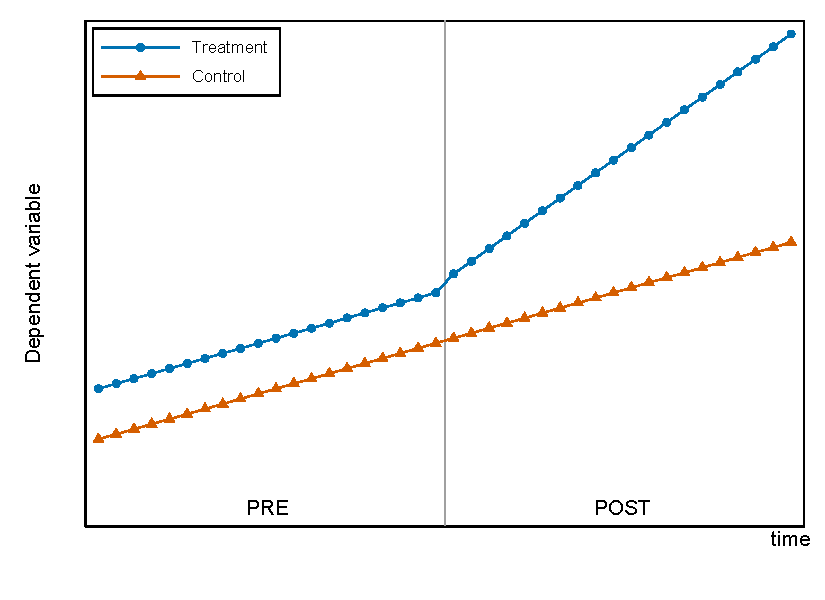
\includegraphics[height=4.0cm]{fig/plainDD2.pdf}};
	
	\node[anchor=north,align=center] (text1) at (fig.south) {When treatment alters time trend (ie slope and not just level)};
	
	\node[anchor=base west,align=left] (text2) at ([xshift=0.25cm,yshift=-0.625cm]text1.base west) {\structure{$\bullet$} DD estimand depends on chosen evaluation window};	
	
	\end{tikzpicture}
\end{center}
\end{frame}



%%%%%%%%%%%%%%%%%%%%%%%%%%%%%%%%%%%%%%%%%%%%%%%%%%%%%%%%%%%%%%%%%%%%%%%

\begin{frame}{The Event Study Approach}

\medskip
Always plot your data (and look for a plot in papers)!

\medskip
\begin{itemize}
	
	\item When common trends holds, diff-in-diff estimator is still unbiased measure of average treatment effect on treated units 
	
	\item Which treatment effect?  Answer: ``impact of $X$ over $\tau$ years''
	
\end{itemize}

\pause
\medskip
\medskip
Alternative is to estimate treatment effect separately for each period

\medskip
\begin{itemize}
	
	\item Include treatment variable interacted with leads and lags
	
	\item Allows for statistical tests of functional form of effect
	
	\item Requires more data (statistical power) than pooled diff-in-diff
	
\end{itemize}

\end{frame}



%%%%%%%%%%%%%%%%%%%%%%%%%%%%%%%%%%%%%%%%%%%%%%%%%%%%%%%%%%%%%%%%%%%%%%%

\begin{frame}<handout:0>{The Event Study Approach}

\begin{center}
	\begin{tikzpicture}
	
	% blank canvas
	\only<handout>{\fill[fill=white,draw=white,ultra thin]
		(0,0) -- (11,0) -- (11,6) -- (0,6) -- cycle;}
	\only<beamer>{\fill[fill=white,draw=white,ultra thin]
		(0,0) -- (14,0) -- (14,6) -- (0,6) -- cycle;}
	\only<beamer>{\draw[draw=oiblue!60,fill=oiblue!10,opacity=0.5] (11,1) rectangle (14,5);}
	%\draw[step=1.0,gray!20,thin] (0,0) grid (11,6);
	
	%	\pgfmathsetmacro\xshift{0.5cm};
	%	\pgfmathsetmacro\yshift{5.5cm};
	%	\pgfmathsetmacro\mycolor{"gray"};
	
	\node[anchor=north west,align=left] (text1) at (0.25,5.75) {Let $Z_{i,1}$ be an indicator for first observation after unit is treated};
	
	\node[anchor=base west,align=left] (text2) at ([xshift=0.25cm,yshift=-0.625cm]text1.base west) {\structure{$\Rightarrow$} $Z_{i,1} = 1$ when $  D_{i,t} = 1$ AND $  D_{i,t-1} = 0$};	
	
	\end{tikzpicture}
\end{center}
\end{frame}


%%%%%%%%%%%%%%%%%%%%%%%%%%%%%%%%%%%%%%%%%%%%%%%%%%%%%%%%%%%%%%%%%%%%%%%

\begin{frame}<handout:0>{The Event Study Approach}

\begin{center}
	\begin{tikzpicture}
	
	% blank canvas
	\only<handout>{\fill[fill=white,draw=white,ultra thin]
		(0,0) -- (11,0) -- (11,6) -- (0,6) -- cycle;}
	\only<beamer>{\fill[fill=white,draw=white,ultra thin]
		(0,0) -- (14,0) -- (14,6) -- (0,6) -- cycle;}
	\only<beamer>{\draw[draw=oiblue!60,fill=oiblue!10,opacity=0.5] (11,1) rectangle (14,5);}
	%\draw[step=1.0,gray!20,thin] (0,0) grid (11,6);
	
	%	\pgfmathsetmacro\xshift{0.5cm};
	%	\pgfmathsetmacro\yshift{5.5cm};
	%	\pgfmathsetmacro\mycolor{"gray"};
	
	\node[anchor=north west,align=left] (text1) at (0.25,5.75) {Let $Z_{i,1}$ be an indicator for first observation after unit is treated};
	
	\node[anchor=base west,align=left] (text2) at ([xshift=0.25cm,yshift=-0.625cm]text1.base west) {\structure{$\Rightarrow$} $Z_{i,1} = 1$ when $  D_{i,t} = 1$ AND $  D_{i,t-1} = 0$};	
	
	\node[anchor=base west,align=left] (text3) at ([xshift=0cm,yshift=-0.625cm]text2.base west) {\structure{$\Rightarrow$} $Z_{i,k} = $ indicator for  the $k^{\textsf{th}}$ period after treatment (starts)};
	
	\node[anchor=base west,align=left] (text4) at ([xshift=0cm,yshift=-0.625cm]text3.base west) {\structure{$\Rightarrow$} $Z_{i,-k} = $ indicator for $k^{\textsf{th}}$ period before treatment starts};	
	
	\end{tikzpicture}
\end{center}
\end{frame}



%%%%%%%%%%%%%%%%%%%%%%%%%%%%%%%%%%%%%%%%%%%%%%%%%%%%%%%%%%%%%%%%%%%%%%%

\begin{frame}{The Event Study Approach}

\begin{center}
	\begin{tikzpicture}
	
	% blank canvas
	\only<handout>{\fill[fill=white,draw=white,ultra thin]
		(0,0) -- (11,0) -- (11,6) -- (0,6) -- cycle;}
	\only<beamer>{\fill[fill=white,draw=white,ultra thin]
		(0,0) -- (14,0) -- (14,6) -- (0,6) -- cycle;}
	\only<beamer>{\draw[draw=oiblue!60,fill=oiblue!10,opacity=0.5] (11,1) rectangle (14,5);}
	%\draw[step=1.0,gray!20,thin] (0,0) grid (11,6);
	
	%	\pgfmathsetmacro\xshift{0.5cm};
	%	\pgfmathsetmacro\yshift{5.5cm};
	%	\pgfmathsetmacro\mycolor{"gray"};
	
	\node[anchor=north west,align=left] (text1) at (0.25,5.75) {Let $Z_{i,1}$ be an indicator for first observation after unit is treated};
	
	\node[anchor=base west,align=left] (text2) at ([xshift=0.25cm,yshift=-0.625cm]text1.base west) {\structure{$\Rightarrow$} $Z_{i,1} = 1$ when $  D_{i,t} = 1$ AND $  D_{i,t-1} = 0$};	
	
	\node[anchor=base west,align=left] (text3) at ([xshift=0cm,yshift=-0.625cm]text2.base west) {\structure{$\Rightarrow$} $Z_{i,k} = $ indicator for  the $k^{\textsf{th}}$ period after treatment (starts)};
	
	\node[anchor=base west,align=left] (text4) at ([xshift=0cm,yshift=-0.625cm]text3.base west) {\structure{$\Rightarrow$} $Z_{i,-k} = $ indicator for $k^{\textsf{th}}$ period before treatment starts};	
	
	\node[anchor=base west,align=left] (text5) at ([xshift=-0.25cm,yshift=-0.875cm]text4.base west) {Event study specification:  };	
	
	\node[anchor=base west,align=left,font=\small] (text6) at ([xshift=0.25cm,yshift=-0.625cm]text5.base west) {$Y_{i,t} = \alpha + \eta_i + \phi_t +  $};	
	\node[anchor=base west,align=left,font=\small] (text7) at ([xshift=0.5cm,yshift=-0.625cm]text6.base west) {$\ldots + \textcolor{red}{\beta_{-2}} Z_{i,-2} +  \textcolor{red}{\beta_{1}}  Z_{i,1}  +  \textcolor{red}{\beta_{2}}  Z_{i,2}  + \ldots + \epsilon_{i,t} $};
	
	\node[anchor=base west,align=left,font=\small] (text8) at ([xshift=-0.75cm,yshift=-0.625cm]text7.base west) {(notice we've omitted dummy for last pre-treatment period)};
	
	\end{tikzpicture}
\end{center}
\end{frame}



%%%%%%%%%%%%%%%%%%%%%%%%%%%%%%%%%%%%%%%%%%%%%%%%%%%%%%%%%%%%%%%%%%%%%%%

\begin{frame}<handout:0>{The Event Study Approach in Stata}

\begin{center}
	\begin{tikzpicture}
	
	% blank canvas
	\only<handout>{\fill[fill=white,draw=white,ultra thin]
		(0,0) -- (11,0) -- (11,6) -- (0,6) -- cycle;}
	\only<beamer>{\fill[fill=white,draw=white,ultra thin]
		(0,0) -- (14,0) -- (14,6) -- (0,6) -- cycle;}
	\only<beamer>{\draw[draw=oiblue!60,fill=oiblue!10,opacity=0.5] (11,1) rectangle (14,5);}
	%\draw[step=1.0,gray!20,thin] (0,0) grid (11,6);
	
	%\node[anchor=north west,align=left] (text1) at (0.25,5.75) {reg y minus3 minus2 minus1 plus1 plus2 plus3 i.time i.id};
	\node[anchor=north west,align=left,red] (text1) at (0.25,5.5) {reg y};
	\node[anchor=base west,align=left,black] (text1b) at ([xshift=-0.125cm]text1.base east) {minus3 minus2 minus1};
	\node[anchor=base west,align=left,black] (text1c) at ([xshift=-0.125cm]text1b.base east) {plus1 plus2 plus3};
	\node[anchor=base west,align=left,black] (text1d) at ([xshift=-0.125cm]text1c.base east) {i.time i.id};
	
	%\node[anchor=base west,align=left] (text2) at ([xshift=0.25cm,yshift=-0.625cm]text1.base west) {\structure{$\Rightarrow$} $Z_{i,1} = 1$ when $  D_{i,t} = 1$ AND $  D_{i,t-1} = 0$};	
	
	\end{tikzpicture}
\end{center}
\end{frame}



%%%%%%%%%%%%%%%%%%%%%%%%%%%%%%%%%%%%%%%%%%%%%%%%%%%%%%%%%%%%%%%%%%%%%%%

\begin{frame}<handout:0>{The Event Study Approach in Stata}

\begin{center}
	\begin{tikzpicture}
	
	% blank canvas
	\only<handout>{\fill[fill=white,draw=white,ultra thin]
		(0,0) -- (11,0) -- (11,6) -- (0,6) -- cycle;}
	\only<beamer>{\fill[fill=white,draw=white,ultra thin]
		(0,0) -- (14,0) -- (14,6) -- (0,6) -- cycle;}
	\only<beamer>{\draw[draw=oiblue!60,fill=oiblue!10,opacity=0.5] (11,1) rectangle (14,5);}
	%\draw[step=1.0,gray!20,thin] (0,0) grid (11,6);
	
	%\node[anchor=north west,align=left] (text1) at (0.25,5.75) {reg y minus3 minus2 minus1 plus1 plus2 plus3 i.time i.id};
	\node[anchor=north west,align=left,black] (text1) at (0.25,5.5) {reg y};
	\node[anchor=base west,align=left,red] (text1b) at ([xshift=-0.125cm]text1.base east) {minus3 minus2 minus1};
	\node[anchor=base west,align=left,black] (text1c) at ([xshift=-0.125cm]text1b.base east) {plus1 plus2 plus3};
	\node[anchor=base west,align=left,black] (text1d) at ([xshift=-0.125cm]text1c.base east) {i.time i.id};
	
	\node[anchor=north,align=center,red] (label) at ([yshift=-0.625cm]text1b.south) {pre-treatment dummies};
	\draw[red,-.>] (label.north) -- (text1b.south);	
	
	\end{tikzpicture}
\end{center}
\end{frame}


%%%%%%%%%%%%%%%%%%%%%%%%%%%%%%%%%%%%%%%%%%%%%%%%%%%%%%%%%%%%%%%%%%%%%%%

\begin{frame}{The Event Study Approach in Stata}

\begin{center}
	\begin{tikzpicture}
	
	% blank canvas
	\only<handout>{\fill[fill=white,draw=white,ultra thin]
		(0,0) -- (11,0) -- (11,6) -- (0,6) -- cycle;}
	\only<beamer>{\fill[fill=white,draw=white,ultra thin]
		(0,0) -- (14,0) -- (14,6) -- (0,6) -- cycle;}
	\only<beamer>{\draw[draw=oiblue!60,fill=oiblue!10,opacity=0.5] (11,1) rectangle (14,5);}
	%\draw[step=1.0,gray!20,thin] (0,0) grid (11,6);
	
	%\node[anchor=north west,align=left] (text1) at (0.25,5.75) {reg y minus3 minus2 minus1 plus1 plus2 plus3 i.time i.id};
	\node[anchor=north west,align=left,black] (text1) at (0.25,5.5) {reg y};
	\node[anchor=base west,align=left,black] (text1b) at ([xshift=-0.125cm]text1.base east) {minus3 minus2 minus1};
	\node[anchor=base west,align=left,red] (text1c) at ([xshift=-0.125cm]text1b.base east) {plus1 plus2 plus3};
	\node[anchor=base west,align=left,black] (text1d) at ([xshift=-0.125cm]text1c.base east) {i.time i.id};
	
	\node[anchor=north,align=center,red] (label) at ([yshift=-0.625cm]text1c.south) {post-treatment dummies};
	\draw[red,-.>] (label.north) -- (text1c.south);	
	
	\end{tikzpicture}
\end{center}
\end{frame}


%%%%%%%%%%%%%%%%%%%%%%%%%%%%%%%%%%%%%%%%%%%%%%%%%%%%%%%%%%%%%%%%%%%%%%%

\begin{frame}{The Event Study Approach in Stata}

\begin{center}
	\begin{tikzpicture}
	
	% blank canvas
	\only<handout>{\fill[fill=white,draw=white,ultra thin]
		(0,0) -- (11,0) -- (11,6) -- (0,6) -- cycle;}
	\only<beamer>{\fill[fill=white,draw=white,ultra thin]
		(0,0) -- (14,0) -- (14,6) -- (0,6) -- cycle;}
	\only<beamer>{\draw[draw=oiblue!60,fill=oiblue!10,opacity=0.5] (11,1) rectangle (14,5);}
	%\draw[step=1.0,gray!20,thin] (0,0) grid (11,6);
	
	%\node[anchor=north west,align=left] (text1) at (0.25,5.75) {reg y minus3 minus2 minus1 plus1 plus2 plus3 i.time i.id};
	\node[anchor=north west,align=left,black] (text1) at (0.25,5.5) {reg y};
	\node[anchor=base west,align=left,black] (text1b) at ([xshift=-0.125cm]text1.base east) {minus3 minus2 minus1};
	\node[anchor=base west,align=left,red] (text1c) at ([xshift=-0.125cm]text1b.base east) {plus1 plus2 plus3};
	\node[anchor=base west,align=left,black] (text1d) at ([xshift=-0.125cm]text1c.base east) {i.time i.id};
	
	\node[anchor=north,align=center,red] (label) at ([yshift=-0.625cm]text1c.south) {post-treatment dummies};
	\draw[red,-.>] (label.north) -- (text1c.south);	
	
	\node[anchor=north west,align=left,black] (text2) at ([yshift=-2.25cm]text1.north west) {Treatment effects relative to omitted ``period zero''};
	\node[anchor=north west,align=left,black] (text3) at ([xshift=0.25cm,yshift=-0.65cm]text2.north west) {\structure{$\Rightarrow$} Exact moment of treatment or last pre-treatment observation};
	
	\end{tikzpicture}
\end{center}
\end{frame}


%%%%%%%%%%%%%%%%%%%%%%%%%%%%%%%%%%%%%%%%%%%%%%%%%%%%%%%%%%%%%%%%%%%%%%%

\begin{frame}<handout:0>{The Event Study Approach in Stata}

\begin{center}
	\begin{tikzpicture}
	
	% blank canvas
	\only<handout>{\fill[fill=white,draw=white,ultra thin]
		(0,0) -- (11,0) -- (11,6) -- (0,6) -- cycle;}
	\only<beamer>{\fill[fill=white,draw=white,ultra thin]
		(0,0) -- (14,0) -- (14,6) -- (0,6) -- cycle;}
	\only<beamer>{\draw[draw=oiblue!60,fill=oiblue!10,opacity=0.5] (11,1) rectangle (14,5);}
	%\draw[step=1.0,gray!20,thin] (0,0) grid (11,6);
	
	%\node[anchor=north west,align=left] (text1) at (0.25,5.75) {reg y minus3 minus2 minus1 plus1 plus2 plus3 i.time i.id};
	\node[anchor=north west,align=left,black] (text1) at (0.25,5.5) {reg y};
	\node[anchor=base west,align=left,black] (text1b) at ([xshift=-0.125cm]text1.base east) {minus3 minus2 minus1};
	\node[anchor=base west,align=left,black] (text1c) at ([xshift=-0.125cm]text1b.base east) {plus1 plus2 plus3};
	\node[anchor=base west,align=left,red] (text1d) at ([xshift=-0.125cm]text1c.base east) {i.time i.id};
	
	\node[anchor=north,align=center,red] (label) at ([yshift=-0.625cm]text1d.south) {fixed effects};
	\draw[red,-.>] (label.north) -- (text1d.south);	
	
	\end{tikzpicture}
\end{center}
\end{frame}



%%%%%%%%%%%%%%%%%%%%%%%%%%%%%%%%%%%%%%%%%%%%%%%%%%%%%%%%%%%%%%%%%%%%%%%

\begin{frame}{The Event Study Approach in Stata}

\begin{center}
	\begin{tikzpicture}
	
	% blank canvas
	\only<handout>{\fill[fill=white,draw=white,ultra thin]
		(0,0) -- (11,0) -- (11,6) -- (0,6) -- cycle;}
	\only<beamer>{\fill[fill=white,draw=white,ultra thin]
		(0,0) -- (14,0) -- (14,6) -- (0,6) -- cycle;}
	\only<beamer>{\draw[draw=oiblue!60,fill=oiblue!10,opacity=0.5] (11,1) rectangle (14,5);}
	%\draw[step=1.0,gray!20,thin] (0,0) grid (11,6);
	
	%	\pgfmathsetmacro\xshift{0.5cm};
	%	\pgfmathsetmacro\yshift{5.5cm};
	%	\pgfmathsetmacro\mycolor{"gray"};
	
	\node[anchor=north] (fig) at (5,5.75) {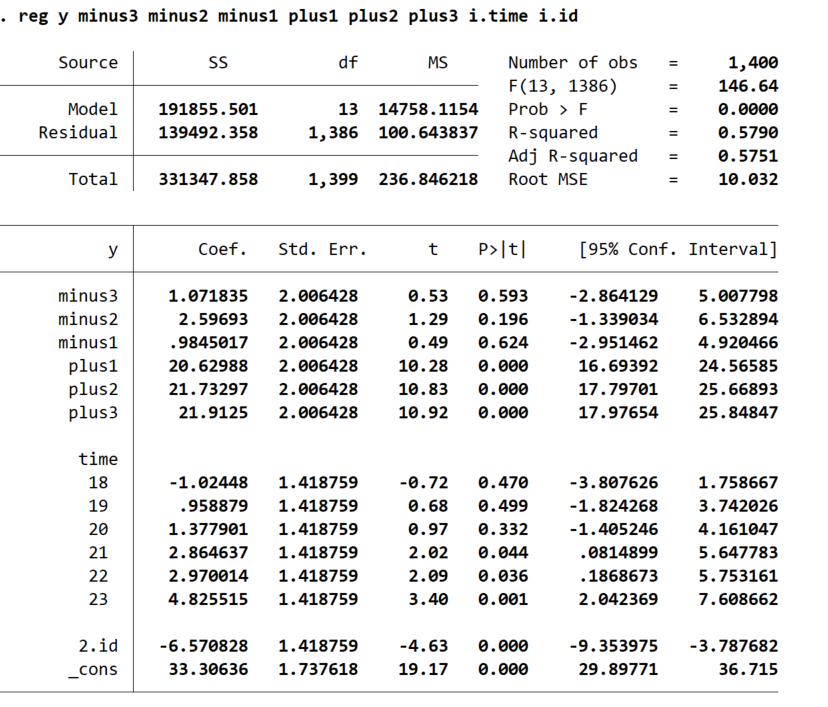
\includegraphics[height=5.2cm]{img/event-stata1.png}};
	
%	\node[anchor=north,align=center] (text1) at (fig.south) {Clear interpretation when treatment effect is constant};
%	
%	\node[anchor=base,align=center] (text2) at ([yshift=-0.625cm]text1.base) {\structure{$\Rightarrow$} $E [ Y_{it} ] = \textcolor{red}{\gamma_i} + \textcolor{red}{\lambda_t} + \delta_i D_{it} $};	
	
	\end{tikzpicture}
\end{center}

\end{frame}


%%%%%%%%%%%%%%%%%%%%%%%%%%%%%%%%%%%%%%%%%%%%%%%%%%%%%%%%%%%%%%%%%%%%%%%

\begin{frame}<handout:0>{The Event Study Approach in Stata}

\begin{center}
	\begin{tikzpicture}
	
	% blank canvas
	\only<handout>{\fill[fill=white,draw=white,ultra thin]
		(0,0) -- (11,0) -- (11,6) -- (0,6) -- cycle;}
	\only<beamer>{\fill[fill=white,draw=white,ultra thin]
		(0,0) -- (14,0) -- (14,6) -- (0,6) -- cycle;}
	\only<beamer>{\draw[draw=oiblue!60,fill=oiblue!10,opacity=0.5] (11,1) rectangle (14,5);}
	%\draw[step=1.0,gray!20,thin] (0,0) grid (11,6);
	
	%	\pgfmathsetmacro\xshift{0.5cm};
	%	\pgfmathsetmacro\yshift{5.5cm};
	%	\pgfmathsetmacro\mycolor{"gray"};
	
	\node[anchor=north] (fig) at (5,5.75) {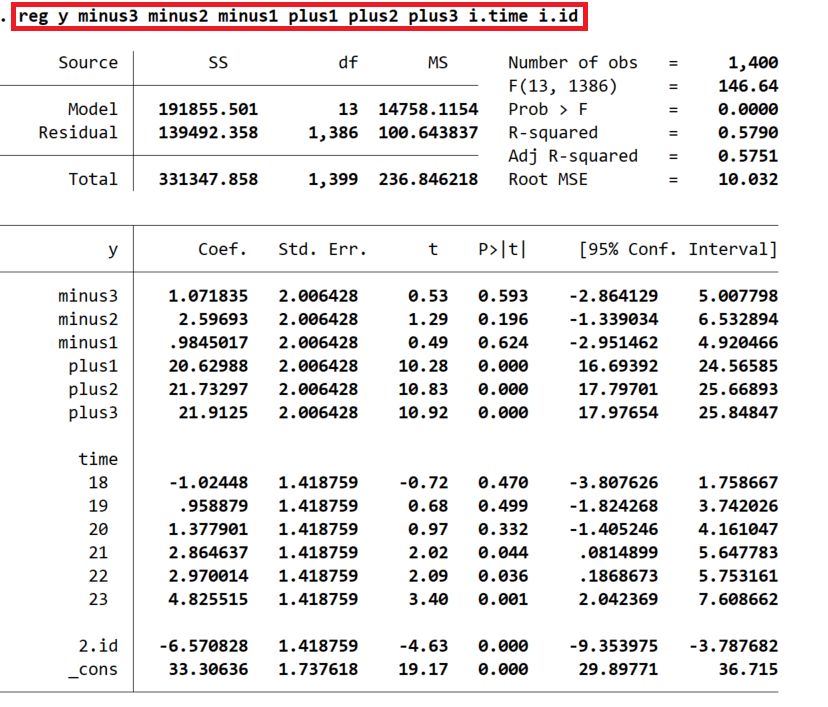
\includegraphics[height=5.2cm]{img/event-stata2.png}};
	
	%	\node[anchor=north,align=center] (text1) at (fig.south) {Clear interpretation when treatment effect is constant};
	%	
	%	\node[anchor=base,align=center] (text2) at ([yshift=-0.625cm]text1.base) {\structure{$\Rightarrow$} $E [ Y_{it} ] = \textcolor{red}{\gamma_i} + \textcolor{red}{\lambda_t} + \delta_i D_{it} $};	
	
	\end{tikzpicture}
\end{center}

\end{frame}


%%%%%%%%%%%%%%%%%%%%%%%%%%%%%%%%%%%%%%%%%%%%%%%%%%%%%%%%%%%%%%%%%%%%%%%

\begin{frame}<handout:0>{The Event Study Approach in Stata}

\begin{center}
	\begin{tikzpicture}
	
	% blank canvas
	\only<handout>{\fill[fill=white,draw=white,ultra thin]
		(0,0) -- (11,0) -- (11,6) -- (0,6) -- cycle;}
	\only<beamer>{\fill[fill=white,draw=white,ultra thin]
		(0,0) -- (14,0) -- (14,6) -- (0,6) -- cycle;}
	\only<beamer>{\draw[draw=oiblue!60,fill=oiblue!10,opacity=0.5] (11,1) rectangle (14,5);}
	%\draw[step=1.0,gray!20,thin] (0,0) grid (11,6);
	
	%	\pgfmathsetmacro\xshift{0.5cm};
	%	\pgfmathsetmacro\yshift{5.5cm};
	%	\pgfmathsetmacro\mycolor{"gray"};
	
	\node[anchor=north] (fig) at (5,5.75) {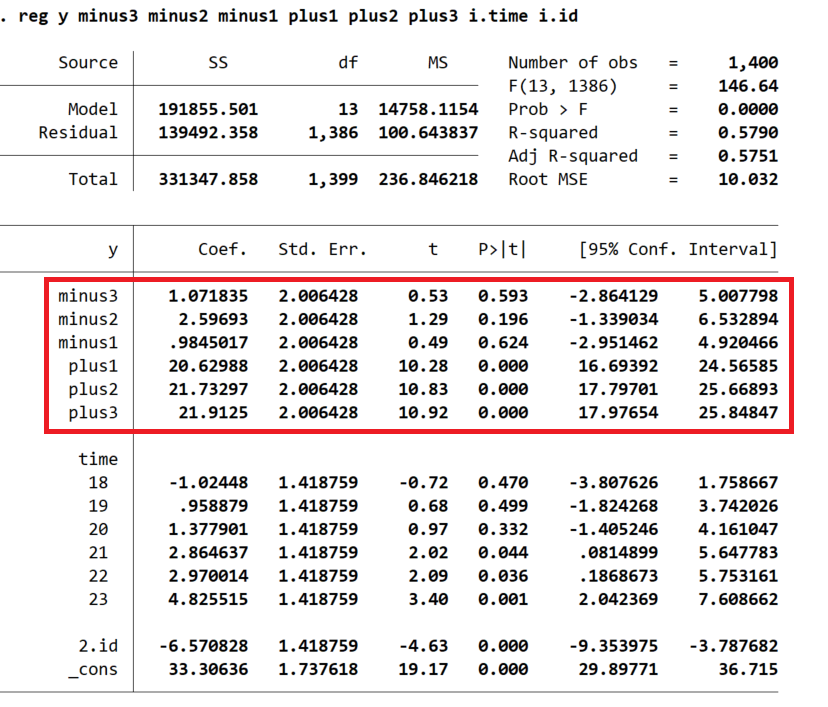
\includegraphics[height=5.2cm]{img/event-stata3.png}};
	
	%	\node[anchor=north,align=center] (text1) at (fig.south) {Clear interpretation when treatment effect is constant};
	%	
	%	\node[anchor=base,align=center] (text2) at ([yshift=-0.625cm]text1.base) {\structure{$\Rightarrow$} $E [ Y_{it} ] = \textcolor{red}{\gamma_i} + \textcolor{red}{\lambda_t} + \delta_i D_{it} $};	
	
	\end{tikzpicture}
\end{center}

\end{frame}


%%%%%%%%%%%%%%%%%%%%%%%%%%%%%%%%%%%%%%%%%%%%%%%%%%%%%%%%%%%%%%%%%%%%%%%

\begin{frame}<handout:0>{The Event Study Approach in Stata}

\begin{center}
	\begin{tikzpicture}
	
	% blank canvas
	\only<handout>{\fill[fill=white,draw=white,ultra thin]
		(0,0) -- (11,0) -- (11,6) -- (0,6) -- cycle;}
	\only<beamer>{\fill[fill=white,draw=white,ultra thin]
		(0,0) -- (14,0) -- (14,6) -- (0,6) -- cycle;}
	\only<beamer>{\draw[draw=oiblue!60,fill=oiblue!10,opacity=0.5] (11,1) rectangle (14,5);}
	%\draw[step=1.0,gray!20,thin] (0,0) grid (11,6);
	
	%	\pgfmathsetmacro\xshift{0.5cm};
	%	\pgfmathsetmacro\yshift{5.5cm};
	%	\pgfmathsetmacro\mycolor{"gray"};
	
	\node[anchor=north] (fig) at (5,5.75) {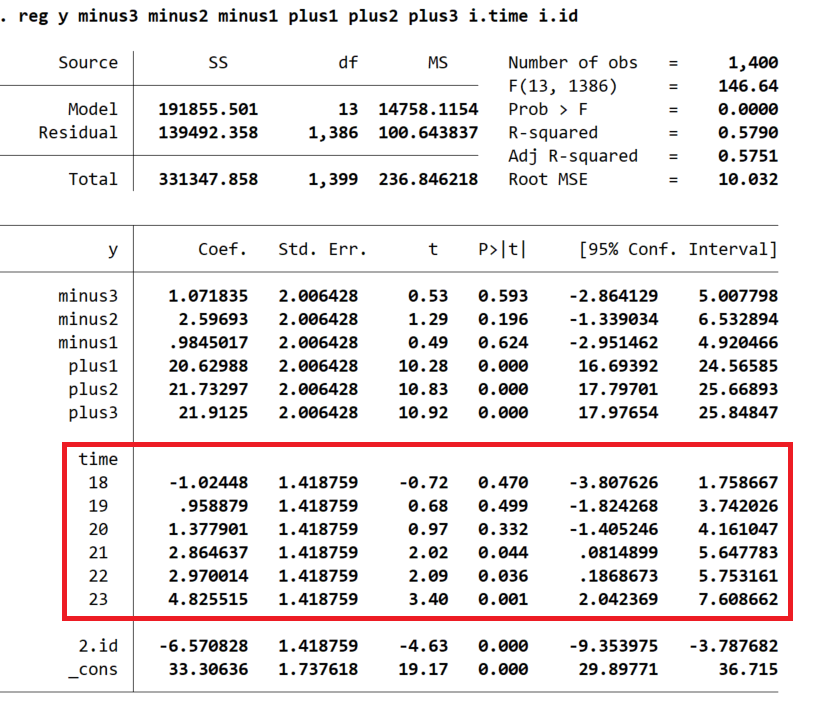
\includegraphics[height=5.2cm]{img/event-stata4.png}};
	
	%	\node[anchor=north,align=center] (text1) at (fig.south) {Clear interpretation when treatment effect is constant};
	%	
	%	\node[anchor=base,align=center] (text2) at ([yshift=-0.625cm]text1.base) {\structure{$\Rightarrow$} $E [ Y_{it} ] = \textcolor{red}{\gamma_i} + \textcolor{red}{\lambda_t} + \delta_i D_{it} $};	
	
	\end{tikzpicture}
\end{center}

\end{frame}


%%%%%%%%%%%%%%%%%%%%%%%%%%%%%%%%%%%%%%%%%%%%%%%%%%%%%%%%%%%%%%%%%%%%%%%

\begin{frame}<handout:0>{The Event Study Approach:  Graphing Your Results}

\begin{center}
	\begin{tikzpicture}
	
	% blank canvas
	\only<handout>{\fill[fill=white,draw=white,ultra thin]
		(0,0) -- (11,0) -- (11,6) -- (0,6) -- cycle;}
	\only<beamer>{\fill[fill=white,draw=white,ultra thin]
		(0,0) -- (14,0) -- (14,6) -- (0,6) -- cycle;}
	\only<beamer>{\draw[draw=oiblue!60,fill=oiblue!10,opacity=0.5] (11,1) rectangle (14,5);}
	%\draw[step=1.0,gray!20,thin] (0,0) grid (11,6);
	
	%	\pgfmathsetmacro\xshift{0.5cm};
	%	\pgfmathsetmacro\yshift{5.5cm};
	%	\pgfmathsetmacro\mycolor{"gray"};
	
	\node[anchor=north] (fig) at (5,5.25) {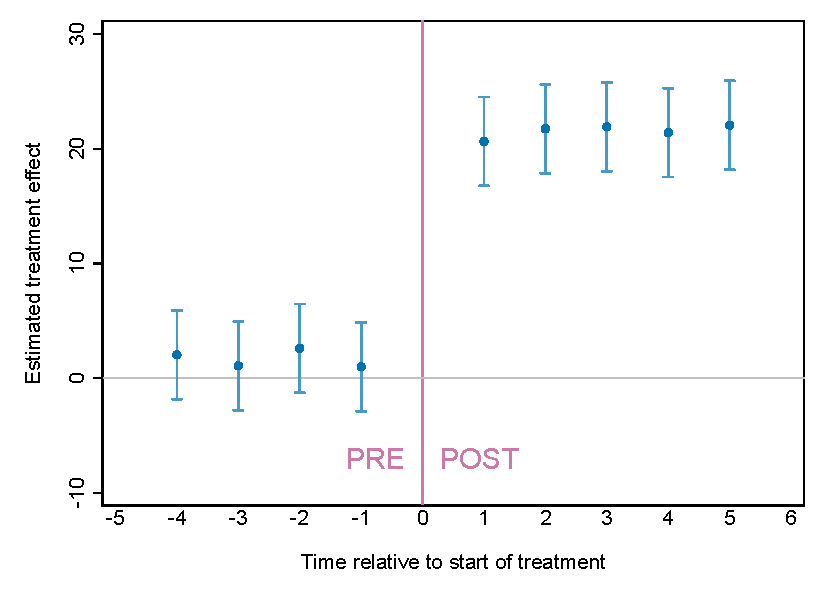
\includegraphics[height=4.8cm]{fig/event-study.pdf}};	
	
	\end{tikzpicture}
\end{center}

\end{frame}


%%%%%%%%%%%%%%%%%%%%%%%%%%%%%%%%%%%%%%%%%%%%%%%%%%%%%%%%%%%%%%%%%%%%%%%

\begin{frame}{The Event Study Approach:  Hypothesis Testing}

Hypotheses one might test in event studies:

\medskip
\begin{itemize}
	
	\item Individual coefficients (e.g.~specific treatment effects) are zero
	
	\item A group of coefficients are all (jointly) equal to zero
	
	\item A group of coefficients are equal to each other (but not zero)
	
	\item A group of coefficients are related to each other linearly
	
\end{itemize}

\medskip
\medskip
In Stata, we can test hypotheses after estimation using \textcolor{blue}{\texttt{test}}:

\medskip
\textcolor{blue}{\texttt{reg y x1 x2 x3 x4}}

\textcolor{blue}{\texttt{test x1 x2 x3 x4}} (list of coefficients)

%\medskip
\textcolor{blue}{\texttt{test x1=x2}} (test of equality)

\end{frame}


%%%%%%%%%%%%%%%%%%%%%%%%%%%%%%%%%%%%%%%%%%%%%%%%%%%%%%%%%%%%%%%%%%%%%%%

\begin{frame}{The Event Study Approach:  Hypothesis Testing}

\begin{center}
	\begin{tikzpicture}
	
	% blank canvas
	\only<handout>{\fill[fill=white,draw=white,ultra thin]
		(0,0) -- (11,0) -- (11,6) -- (0,6) -- cycle;}
	\only<beamer>{\fill[fill=white,draw=white,ultra thin]
		(0,0) -- (14,0) -- (14,6) -- (0,6) -- cycle;}
	\only<beamer>{\draw[draw=oiblue!60,fill=oiblue!10,opacity=0.5] (11,1) rectangle (14,5);}
	%\draw[step=1.0,gray!20,thin] (0,0) grid (11,6);
	
	%	\pgfmathsetmacro\xshift{0.5cm};
	%	\pgfmathsetmacro\yshift{5.5cm};
	%	\pgfmathsetmacro\mycolor{"gray"};
	
	\node[anchor=north] (fig) at (5,5.75) {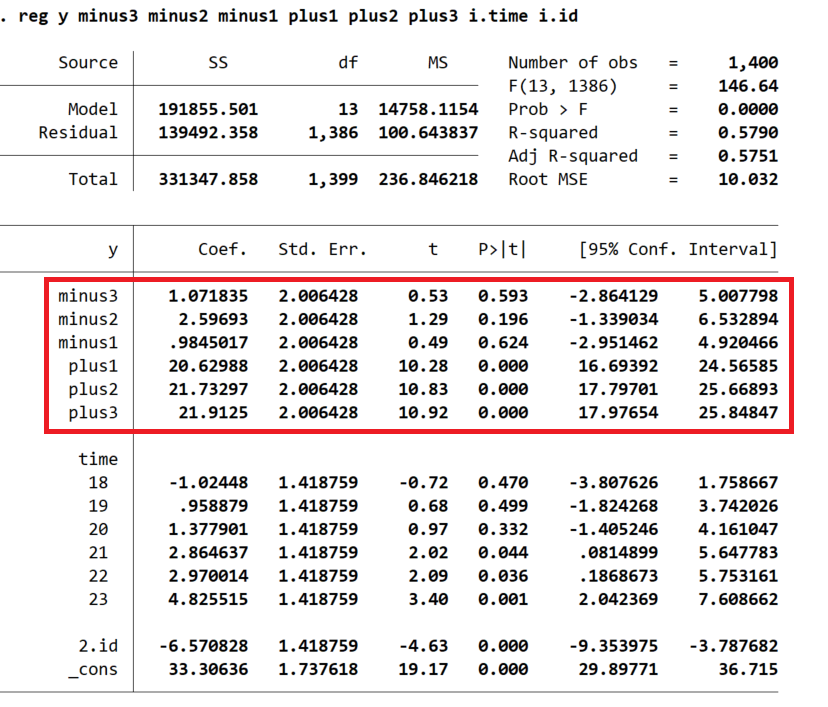
\includegraphics[height=5.2cm]{img/event-stata3.png}};
	
	\end{tikzpicture}
\end{center}

\end{frame}



%%%%%%%%%%%%%%%%%%%%%%%%%%%%%%%%%%%%%%%%%%%%%%%%%%%%%%%%%%%%%%%%%%%%%%%

\begin{frame}{The Event Study Approach:  Hypothesis Testing}

\begin{small}
\textcolor{blue}{\texttt{test minus1 minus2 minus3}} \\

\medskip

\textcolor{blue}{\texttt{( 1)  minus1 = 0}} \\
\textcolor{blue}{\texttt{( 2)  minus2 = 0}} \\
\textcolor{blue}{\texttt{( 3)  minus3 = 0}} \\

\medskip
\textcolor{blue}{\texttt{$\ \ \ \ $F(3,1386) =    0.57}} \\
\textcolor{blue}{\texttt{$\ \ \ \ $Prob $>$ F =    0.6341}} 

\end{small}

\medskip
\medskip

$\Rightarrow$ Particularly useful in testing for pre-treatment common trends
\end{frame}


%%%%%%%%%%%%%%%%%%%%%%%%%%%%%%%%%%%%%%%%%%%%%%%%%%%%%%%%%%%%%%%%%%%%%%%

\begin{frame}{The Event Study Approach:  Hypothesis Testing}

\begin{center}
	\begin{tikzpicture}
	
	% blank canvas
	\only<handout>{\fill[fill=white,draw=white,ultra thin]
		(0,0) -- (11,0) -- (11,6) -- (0,6) -- cycle;}
	\only<beamer>{\fill[fill=white,draw=white,ultra thin]
		(0,0) -- (14,0) -- (14,6) -- (0,6) -- cycle;}
	\only<beamer>{\draw[draw=oiblue!60,fill=oiblue!10,opacity=0.5] (11,1) rectangle (14,5);}
	%\draw[step=1.0,gray!20,thin] (0,0) grid (11,6);
	
	\node[anchor=north] (fig) at (5,5.75) {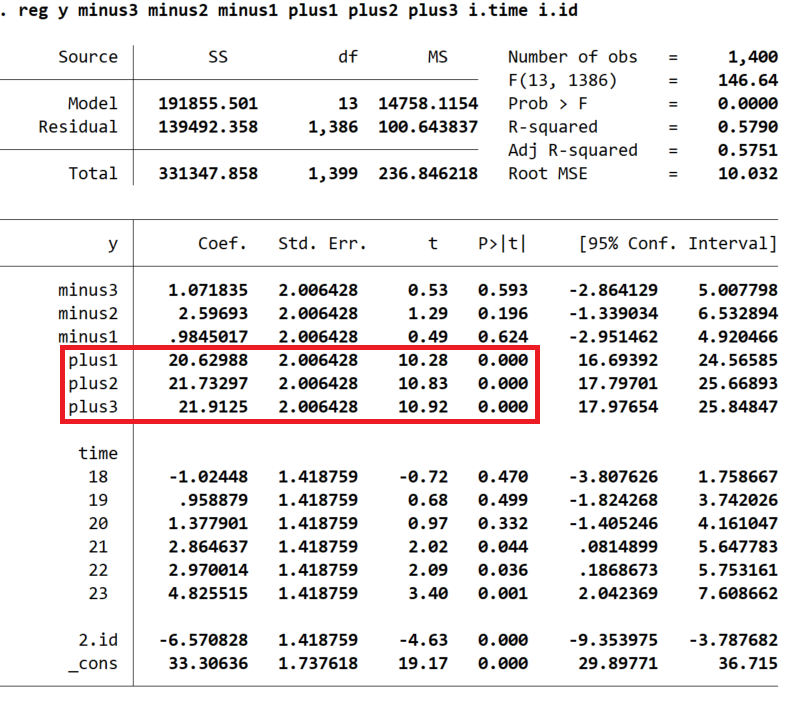
\includegraphics[height=5.2cm]{img/event-stata5.png}};	
	
	\end{tikzpicture}
\end{center}

\end{frame}


%%%%%%%%%%%%%%%%%%%%%%%%%%%%%%%%%%%%%%%%%%%%%%%%%%%%%%%%%%%%%%%%%%%%%%%

\begin{frame}{The Event Study Approach:  Hypothesis Testing}

\begin{small}
	\textcolor{blue}{\texttt{test plus1 = plus2 = plus3}} \\
	
	\medskip
	
	\textcolor{blue}{\texttt{( 1)  plus1 - plus2 = 0}} \\
	\textcolor{blue}{\texttt{( 2)  plus1 - plus3 = 0}} \\
	
	\medskip
	\textcolor{blue}{\texttt{$\ \ \ \ $F(  2,  1386) =    0.24}} \\
	\textcolor{blue}{\texttt{$\ \ \ \ $Prob $>$ F =    0.7869}} 
	
\end{small}

\medskip
\medskip

$\Rightarrow$ Each coefficient statistically significantly different from zero

\medskip

$\Rightarrow$ Coefficients not significantly different from each other
\end{frame}



%%%%%%%%%%%%%%%%%%%%%%%%%%%%%%%%%%%%%%%%%%%%%%%%%%%%%%%%%%%%%%%%%%%%%%%

\begin{frame}{The Event Study Approach:  Hypothesis Testing}

\begin{center}
	\begin{tikzpicture}
	
	% blank canvas
	\only<handout>{\fill[fill=white,draw=white,ultra thin]
		(0,0) -- (11,0) -- (11,6) -- (0,6) -- cycle;}
	\only<beamer>{\fill[fill=white,draw=white,ultra thin]
		(0,0) -- (14,0) -- (14,6) -- (0,6) -- cycle;}
	\only<beamer>{\draw[draw=oiblue!60,fill=oiblue!10,opacity=0.5] (11,1) rectangle (14,5);}
	%\draw[step=1.0,gray!20,thin] (0,0) grid (11,6);

	
	\node[anchor=north] (fig) at (5,5.75) {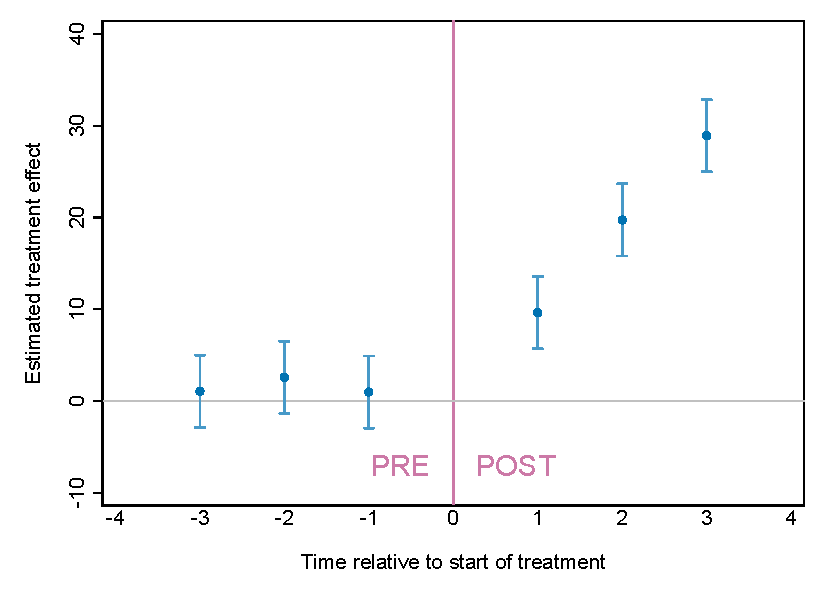
\includegraphics[height=4.8cm]{fig/event-study-slope.pdf}};
		
	
	\end{tikzpicture}
\end{center}

\end{frame}




%%%%%%%%%%%%%%%%%%%%%%%%%%%%%%%%%%%%%%%%%%%%%%%%%%%%%%%%%%%%%%%%%%%%%%%

\begin{frame}{The Event Study Approach:  Hypothesis Testing}

\begin{center}
	\begin{tikzpicture}
	
	% blank canvas
	\only<handout>{\fill[fill=white,draw=white,ultra thin]
		(0,0) -- (11,0) -- (11,6) -- (0,6) -- cycle;}
	\only<beamer>{\fill[fill=white,draw=white,ultra thin]
		(0,0) -- (14,0) -- (14,6) -- (0,6) -- cycle;}
	\only<beamer>{\draw[draw=oiblue!60,fill=oiblue!10,opacity=0.5] (11,1) rectangle (14,5);}
	%\draw[step=1.0,gray!20,thin] (0,0) grid (11,6);
	
	
	\node[anchor=north] (fig) at (5,5.75) {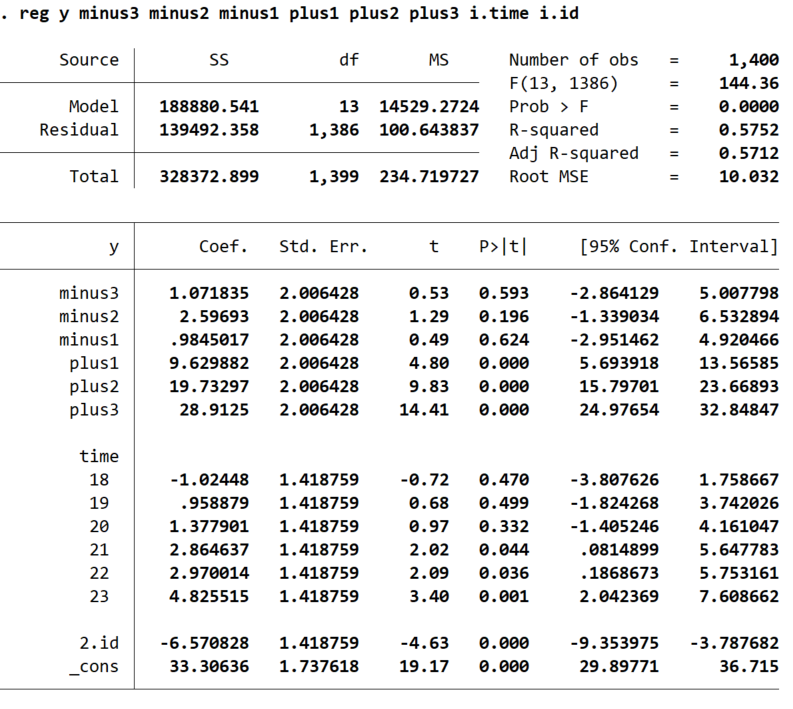
\includegraphics[height=5.2cm]{img/event-slope1.png}};
	
	\end{tikzpicture}
\end{center}

\end{frame}



%%%%%%%%%%%%%%%%%%%%%%%%%%%%%%%%%%%%%%%%%%%%%%%%%%%%%%%%%%%%%%%%%%%%%%%

\begin{frame}<handout:0>{The Event Study Approach:  Hypothesis Testing}

\begin{center}
	\begin{tikzpicture}
	
	% blank canvas
	\only<handout>{\fill[fill=white,draw=white,ultra thin]
		(0,0) -- (11,0) -- (11,6) -- (0,6) -- cycle;}
	\only<beamer>{\fill[fill=white,draw=white,ultra thin]
		(0,0) -- (14,0) -- (14,6) -- (0,6) -- cycle;}
	\only<beamer>{\draw[draw=oiblue!60,fill=oiblue!10,opacity=0.5] (11,1) rectangle (14,5);}
	%\draw[step=1.0,gray!20,thin] (0,0) grid (11,6);
	
	
	\node[anchor=north] (fig) at (5,5.75) {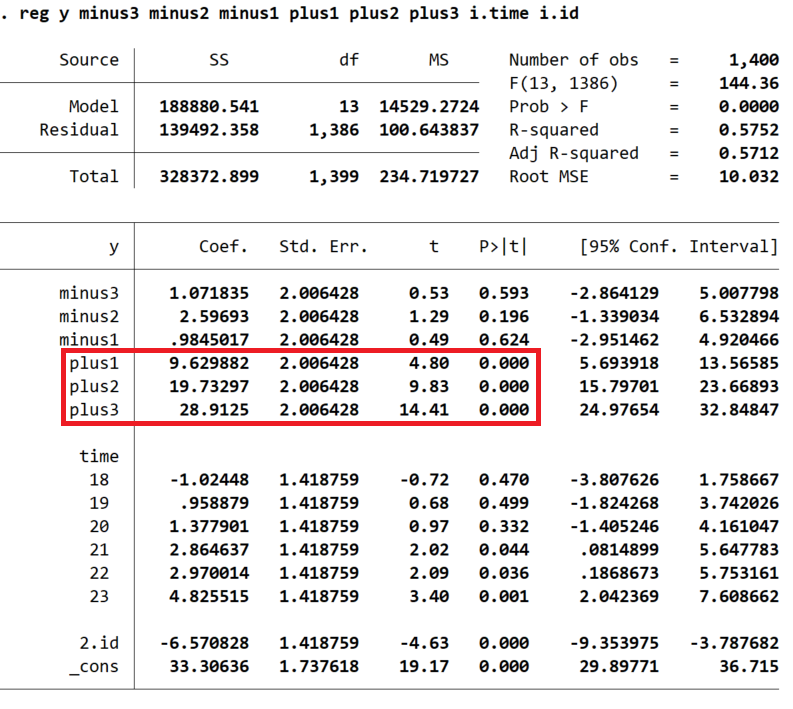
\includegraphics[height=5.2cm]{img/event-slope2.png}};
	
	\end{tikzpicture}
\end{center}

\end{frame}



%%%%%%%%%%%%%%%%%%%%%%%%%%%%%%%%%%%%%%%%%%%%%%%%%%%%%%%%%%%%%%%%%%%%%%%

\begin{frame}{The Event Study Approach:  Hypothesis Testing}

\medskip
Coefficients on \textcolor{blue}{\texttt{plus1}} and \textcolor{blue}{\texttt{plus2}} are not equal: \\

\medskip

\begin{small}
	\textcolor{blue}{\texttt{test plus1 = plus2}} \\
	
	\medskip
	
	\textcolor{blue}{\texttt{( 1)  plus1 - plus2 = 0}} \\
	
	\medskip
	\textcolor{blue}{\texttt{$\ \ \ \ $F(  1,  1386) =   25.35}} \\
	\textcolor{blue}{\texttt{$\ \ \ \ $Prob $>$ F =    0.0000}} 
	
\end{small}

\pause
\medskip
\medskip
Can we reject hypothesis that \textcolor{blue}{\texttt{plus2}} is twice as large as \textcolor{blue}{\texttt{plus1}}? \\

\medskip

\begin{small}
	\textcolor{blue}{\texttt{test 2*plus1 = plus2}} \\
	
	\medskip
	
	\textcolor{blue}{\texttt{( 1)  2*plus1 - plus2 = 0}} \\
	
	\medskip
	\textcolor{blue}{\texttt{$\ \ \ \ $F(  1,  1386) =    0.02}} \\
	\textcolor{blue}{\texttt{$\ \ \ \ $Prob $>$ F =    0.8917}} 
	
\end{small}

\end{frame}


%%%%%%%%%%%%%%%%%%%%%%%%%%%%%%%%%%%%%%%%%%%%%%%%%%%%%%%%%%%%%%%%%%%%%%%%%%%

%\begin{frame}<handout:0>[bg,plain]
\begin{frame}[plain]

\only<beamer>{\begin{adjustwidth}{0cm}{-4cm}}
	
	\begin{center}
		
		\Large{\textcolor{williams}{The end!}}
		
	\end{center}
	
	\only<beamer>{\end{adjustwidth}}
\end{frame}




\end{document}